\documentclass[12pt,a4paper]{article}

% Mathematics
\usepackage{amsmath,amssymb,amsthm,mathtools}

% Typography and layout
\usepackage[utf8]{inputenc}
\usepackage[T1]{fontenc}
\usepackage{lmodern}
\usepackage[margin=1in]{geometry}
\usepackage{setspace}
\onehalfspacing
\usepackage{titlesec}
\titleformat{\section}[block]{\normalsize\bfseries\centering}{\thesection.}{0.5em}{}
\titleformat{\subsection}[block]{\normalsize\itshape\centering}{\thesubsection.}{0.5em}{}

% Tables and figures
\usepackage{booktabs,array,multirow,float,tabularx}
\usepackage{graphicx}

% Colour and links
\usepackage[dvipsnames]{xcolor}
\usepackage[round,sort&compress]{natbib}
\usepackage{hyperref}
\hypersetup{colorlinks=true,linkcolor=blue!60!black,citecolor=blue!60!black,urlcolor=blue!60!black}

% Page numbering
\usepackage{lastpage}
\usepackage{fancyhdr}
\pagestyle{fancy}
\fancyhf{}
\rfoot{\thepage}
\renewcommand{\headrulewidth}{0pt}

% Theorem environments
\newtheorem{proposition}{Proposition}
\newtheorem{corollary}{Corollary}
\newtheorem{definition}{Definition}
\newtheorem{assumption}{Assumption}
\newtheorem{lemma}{Lemma}
\newtheorem{prediction}{Empirical Prediction}
\newtheorem{remark}{Remark}

% Custom commands
\newcommand{\R}{\mathbb{R}}
\newcommand{\E}{\mathbb{E}}
\newcommand{\indic}{\mathbb{1}}
\newcommand{\btheta}{\boldsymbol{\theta}}
\newcommand{\bW}{\mathbf{W}}

\title{\large\textbf{When Coal Retires: A Network Channel for the Carbon Premium}\vspace{-0.5em}}
\author{\normalsize Jose Luis Resendiz\\[4pt] \small Smith School of Enterprise and the Environment, University of Oxford}
\date{\small\today}

\begin{document}
{\singlespacing\maketitle}

\begin{quotation}\small\singlespacing\noindent
\textbf{Abstract.} When a coal plant retires, technologically similar utilities reprice. A one-standard-deviation increase in fuel-mix similarity to a retiring firm predicts a 2.2 percentage point decline in four-month cumulative abnormal returns; geographic proximity is indistinguishable from zero. The channel falls silent in the United States, where retirements are routine, and is strongest in firms with concentrated ownership across both US and non-US sub-samples. Built from public plant registries covering 703 listed utilities across 80 countries, fuel-mix similarity recovers the network structure underneath the carbon premium and prices firms that ESG coverage misses.
\end{quotation}

\medskip\noindent\textit{JEL Classification:} G12, G14, Q54, L94.\\
\noindent\textit{Keywords:} transition risk, stranded assets, fuel-mix similarity, technology networks.

%----------------------------------------------------------------------
\section{Introduction}\label{sec:intro}
%----------------------------------------------------------------------

Coal capacity is retiring at record speed in some jurisdictions and expanding at record speed in others. Listed power utilities operate plants on both sides of that divergence and trade in the same global capital markets, so their cost of capital depends on how those markets price the technological obsolescence revealed each time a coal plant closes. Over 80 percent of known coal reserves must remain unextracted if Paris targets bind \citep{McGlade2015}, placing trillions of dollars in generating assets at risk \citep{Dietz2016}. Stranding fossil-fuel assets imposes macroeconomic costs \citep{MercurePollittVinualesEdwards2018}, and the losses fall disproportionately on investors in advanced economies \citep{SemieniukHoldenMercureSalas2022}. Falling renewable costs and gas prices have already accelerated coal retirements in liberalised electricity markets \citep{FellKaffine2018}. The transition is happening unevenly. Listed power utilities are a natural laboratory for studying how transition shocks transmit between firms: their generation portfolios are observable from public plant registries, their retirement events are dated, and their population is finite. \citet{BoltonKacperczyk2023} document a global carbon premium across 14{,}400 firms in 77 countries, with magnitudes that rise in stricter policy environments. The premium's \emph{propagation}, the channel through which a transition shock at one firm transmits to others, has not been measured.

Measuring propagation is harder than measuring the level of the carbon premium. Existing firm-level transition-risk indicators (emission intensity, ESG scores, climate-text exposure) reduce to scalars; propagation requires a \emph{pairwise} measure of how much one firm's exposure overlaps with another's. The two natural pairwise channels differ in their unit of analysis. Geographic competition for residual demand operates at the local-electricity-market level: when a coal plant exits in one market, its rivals there gain market share. Technology obsolescence operates at the plant level: when coal becomes uneconomic in one jurisdiction, every coal plant globally faces the same revaluation. Both must aggregate to the firm level to enter equity returns, and they aggregate differently. This paper measures the propagation channel in listed power utilities. Using plant-level data on 703 firms across 80 countries and 175 first-mover coal-retirement events, I show that a one-standard-deviation increase in fuel-mix similarity to a retiring firm predicts a 2.2 percentage point decline in four-month cumulative abnormal returns; geographic proximity is indistinguishable from zero. The channel falls silent in the United States, where retirements are routine, and is strongest in firms with concentrated ownership across both US and non-US sub-samples. Built from public plant registries, fuel-mix similarity recovers the network structure underneath the carbon premium.

This network structure follows from a simple aggregation argument. A listed utility typically operates plants in multiple local electricity markets. When a nearby competitor exits, the utility gains market share in that local market, but these local gains are independent across markets and diversify away in the firm's aggregate stock price, much as idiosyncratic sectoral shocks wash out in a balanced production network \citep{AcemogluCarvalhoOzdaglarTahbazSalehi2012}. Technology exposure operates differently: if coal becomes uneconomic in one jurisdiction, every plant using coal faces the same obsolescence risk, regardless of where it is located. Fuel-mix similarity is a common factor that does not diversify. Section~\ref{sec:model} formalises this asymmetry, which I label \emph{asymmetric aggregation}. I construct fuel-mix similarity as the $L_1$ similarity of capacity-share vectors from the Global Energy Monitor, adapting \citet{HobergPhillips2016}'s product-space proximity from text-based 10-K vocabulary to fuel-type capacity shares.

With this similarity in hand, the cross-sectional design fits the exposure framework of \citet{BorusyakHullJaravel2022}: pre-determined fuel-mix shares serve as exposure, each retirement event serves as the shock, and the regression coefficient identifies the dose-response of abnormal returns to technology exposure. The identifying variation is the cross-sectional spread in fuel-mix similarity to a retiring firm, holding the event itself fixed. The shocks are 175 first-mover coal retirements spanning 35 countries, dated from regulatory filings in the Global Energy Monitor. I pre-determine the exposure shares by restricting to plants commissioned before each event, and I also use a stricter pre-2014-vintage cut as a robustness check. Three of the most consequential threats deserve explicit treatment. First, anticipation: if markets price the retirement before its formal date, abnormal returns measured around the event understate the channel. A daily event-time path covering twenty trading days before each retirement bounds the anticipation drift. Second, factor-loading absorption: a new factor candidate may re-load on size, value, or industry exposures. Under multi-factor (Fama-French three-factor plus sample-constructed utility-industry) abnormal-return adjustment the coefficient shrinks by 35 percent but remains significant ($t = -4.50$), placing roughly two-thirds of the loading orthogonal to the four-factor model. Third, parallel-trends violations: a placebo-window \citet{RambachanRoth2023} sensitivity analysis shows the headline tolerates violations up to $1.26\times$ the largest pre-period deviation under single-factor adjustment, satisfying the standard Honest-DID convention (the multi-factor analogue is $0.62\times$). The pricing effect survives event-clustered, two-way (event $\times$ firm) clustered, and Fama-MacBeth Newey-West inference, plus a Romano-Wolf step-down correction across the three primary hypotheses. A leave-one-event-out sensitivity confirms that no single retirement dominates. The \citet{Oster2019} stability bound implies that unobservables would need to be 36 times more important than observables to overturn the result.

The headline coefficient masks two layers of heterogeneity. Across markets, the pricing effect concentrates where coal retirement remains novel and falls silent in the United States, where retirements are routine. Two split-sample tests narrow the candidate explanations for the US null at the country level. A within-US split between restructured retail markets and rate-of-return-regulated states does not support the regulation hypothesis: the channel is at least as strong in regulated states. A non-US developed-versus-emerging split shows the effect is strongest in developed-ex-US markets, weakening informational-efficiency and ownership-structure explanations at the country level. Saturation remains as the most parsimonious country-level explanation: where coal retirement is routine, each new event carries little incremental information about technology viability. At the firm level, however, the US null masks a sharply negative T3 and a sign-reversed T1, and institutional-ownership heterogeneity is the proximate mechanism. Within firms, the channel is strongest in those with concentrated ownership across both sub-samples: in the highest tercile of US 13F manager Herfindahl, $\hat\gamma_{\mathrm{fuel}} = -6.08$ ($t = -3.27$); in the highest tercile of non-US Refinitiv free-float concentration, $\hat\gamma_{\mathrm{fuel}} = -10.90$ ($t = -5.45$), more than twice the full-panel headline. The technology-propagation channel transmits globally where ownership is concentrated. A daily event study covering twenty trading days around each retirement traces a four-phase cumulative-AR path: pre-event drift, announcement reaction, post-announcement recovery, and long-horizon resumption; a randomization placebo on event timing isolates an announcement-specific component beyond the secular carbon-premium baseline. Finally, fuel-mix similarity expands the universe of measurably transition-risk-priced firms: in the subsample where ESG environmental scores are available, both measures survive a joint Fama-MacBeth test (Wald $\chi^2_2 = 25.9$, $p < 0.001$); only 153 of the 565 firms in the operational regression panel carry an environmental score from LSEG Eikon. Fuel-mix similarity, constructed from public plant registries, extends transition-risk measurement to the remaining 412 firms, a 3.7-fold expansion of the panel of firms in which transition risk can be priced.

These results speak to a question that arises whenever climate policy is unilateral: whether countries that delay retiring fossil capacity remain insulated when others move first. The asset-pricing evidence says they do not, in jurisdictions where coal retirement remains uncommon: the market penalises coal-heavy utilities in proportion to their fuel-mix similarity to the retiring firm. The strength of the propagation signal depends on market context, but its financial reach extends well beyond the country where the retirement occurs.

In conversation with prior work, this paper sits at the intersection of three asset-pricing literatures. First, the carbon-premium literature: \citet{BoltonKacperczyk2023}, \citet{PastorStambaughTaylor2022}, and \citet{HsuLiTsou2023} treat the premium as a \emph{level} property of the cross-section, while the fuel-mix network identifies the propagation kernel underneath. Second, firm-level transition-risk measurement: leading approaches extract exposure from corporate text \citep{SautnerVanLentVilkovZhang2023, EngleGiglioKellyLeeStroebel2020} or aggregate emissions intensity into a tradeable factor \citep{GorgenJacobNerlingerRiordanRohlederWilkens2020, PastorStambaughTaylor2021}; fuel-mix similarity differs in being constructed without disclosure or text mining and in capturing \emph{pairwise} technology proximity rather than firm-level intensity. Option-implied measures of climate tail risk \citep{IlhanSautnerVilkov2021} are complementary, picking up extreme events that the fuel-mix factor does not. Third, the network-propagation framework of \citet{AcemogluCarvalhoOzdaglarTahbazSalehi2012}, applied here to a network defined by shared generation technology rather than input-output linkages; the contagion-versus-competition decomposition builds on \citet{LangStulz1992} and \citet{JorionZhang2007}.

The remainder of the paper proceeds as follows. Section~\ref{sec:model} formalises the asymmetric-aggregation framework. Section~\ref{sec:empirical} describes the cross-sectional design and the inference battery. Section~\ref{sec:results} presents the headline pricing results, the daily event study, and the heterogeneity tests. Section~\ref{sec:discussion} interprets the cross-country pattern and the role of institutional ownership. Section~\ref{sec:conclusion} concludes.


%----------------------------------------------------------------------
\section{A Conceptual Framework for Networked Transition Risk}\label{sec:model}
%----------------------------------------------------------------------

When a power utility retires a fossil plant, two consequences follow. Locally, competitors gain market share as residual demand shifts to remaining generators. Globally, every firm using similar technology faces a repricing of its obsolescence risk. These two consequences aggregate to the stock level in different ways. The local effect diversifies across markets. The technology effect does not. This section formalises the asymmetry and derives the estimating equation.

\subsection{Environment}\label{sec:environment}

Consider $N$ listed power utilities indexed by $i$ and a representative risk-averse investor with a monotone stochastic discount factor $m_{1,2} > 0$. Time has three dates: $t=0$ (ex ante), $t=1$ (signal), $t=2$ (payoff). At $t=1$, a subset of firms retire fossil capacity; the vector $\mathbf{s} \geq 0$ records each retirement.

Firm $i$ operates plants in $K_i \geq 1$ local electricity markets, with revenue share $\theta_{ik}$ in market $k$ ($\sum_k \theta_{ik} = 1$). Firms are connected through two row-normalised adjacency matrices. The first, $w^{\text{geo}}_{ij}$, measures geographic proximity between capacity-weighted plant centroids. The second, $w^{\text{fuel}}_{ij}$, measures fuel-mix similarity from the $L_1$ distance between capacity-share vectors. The two matrices differ in a property that proves consequential: geographic proximity varies at the plant level, while fuel-mix similarity is defined over the firm's entire generation portfolio.

Firm $i$'s terminal cash flow is:
\begin{equation}\label{eq:cashflows}
    \Pi_i = \bar{\Pi} + \sum_{k=1}^{K_i} \theta_{ik}\, G_{ik}(\mathbf{s}) \;-\; \psi_i(\alpha_i, \mathbf{s}) + \eta_i,
\end{equation}
where $\bar{\Pi} > 0$ is baseline profitability, $G_{ik}$ captures the competitive benefit in local market $k$, $\psi_i$ is a technology obsolescence penalty, and $\eta_i$ is mean-zero idiosyncratic noise. The two middle terms formalise the two consequences of a restructuring shock.

\subsection{Two Assumptions}\label{sec:channels}

\begin{assumption}[Geographic gains are local]\label{ass:competition}
    When firm $j$ retires capacity $s_j$, the competitive benefit to firm $i$ in market $k$ is $G_{ik}(\mathbf{s}) = \delta \sum_j w^{\mathrm{geo},k}_{ij}\, s_j$ with $\delta > 0$, where $w^{\mathrm{geo},k}_{ij}$ measures proximity in market $k$ specifically. The gains $G_{ik}$ and $G_{ik'}$ are independent across markets $k \neq k'$.
\end{assumption}

\begin{assumption}[Technology obsolescence originates at the plant level]\label{ass:obsolescence}
    Each plant of technology type $\tau$ faces an obsolescence penalty $\phi_\tau \geq 0$ proportional to the signal that $\tau$ is losing economic viability. Retirement shocks reveal information about coal technology specifically, so $\phi_{\mathrm{coal}} = \phi > 0$ and $\phi_\tau = 0$ for non-coal types. Aggregating to the firm level, the technology penalty for firm $i$ is the capacity-weighted sum of its plant-level penalties:
    \begin{equation}\label{eq:obsolescence}
        \psi_i(\alpha_i, \mathbf{s}) = \sum_\tau \frac{\mathrm{MW}_{i\tau}}{\mathrm{MW}_i}\,\phi_\tau \left(1 + \sum_{j} w^{\mathrm{fuel}}_{ij}\, s_j\right) = \phi\,\alpha_i\!\left(1 + \sum_{j} w^{\mathrm{fuel}}_{ij}\, s_j\right),
    \end{equation}
    where $\alpha_i = \mathrm{MW}_{i,\mathrm{coal}} / \mathrm{MW}_i \in [0,1]$ is firm $i$'s coal share and the second equality follows because only coal carries a positive penalty. The firm-level common factor is therefore a derived consequence of plant-level primitives, not a separate assumption.
\end{assumption}

The first assumption is standard: a rival's exit raises residual demand for remaining local generators \citep{DavisHausman2016}. The independence condition captures the fact that local grids serve geographically segmented markets. The second assumption starts from plant-level technology penalties and derives the firm-level obsolescence factor by capacity-weighted aggregation. The economic content is that retirements reveal that a generation technology is losing viability, and the penalty falls on each plant using that technology in proportion to signal strength. Because only coal plants carry a positive penalty, the firm-level exposure reduces to $\alpha_i \cdot \phi$: a firm's coal share is a sufficient statistic for its own-technology vulnerability.

The cross-sectional regression in Section~\ref{sec:empirical} identifies the product $A\phi\bar\alpha$ (with $\bar\alpha$ the sample-mean coal share) rather than $\phi$ in isolation; this combined object suffices for the comparative test of fuel-versus-geographic transmission.

The linear specification $\psi_i = \phi\,\alpha_i(\cdot)$ is a restriction. If penalties are convex in coal share, high-$\alpha$ firms face disproportionately larger losses than the linear model implies. I test for such nonlinearity in the robustness section by including $\alpha_i^2$ interactions.

The obsolescence parameter $\phi$ appears as a structural primitive in Assumption~\ref{ass:obsolescence}, but it is best understood as a reduced-form composite of several economic forces.

\begin{remark}[Interpretation of $\phi$]\label{rem:phi_interpretation}
The obsolescence parameter $\phi$ absorbs the joint price of three economic forces that retirement events transmit. First, expected fiscal carbon-tax adjustments that raise the marginal cost of coal generation. Second, stranded-asset option values that rise as retirement signals shorten the expected useful life of the fleet. Third, demand-side preference shifts that reduce the value of coal-generated electricity. The model treats the composite as a primitive; the empirical work identifies the product $A\phi\bar{\alpha}$ rather than its components separately (Section~\ref{sec:bridge}).
\end{remark}

\subsection{Aggregation}\label{sec:aggregation}

The geographic and technology channels enter equation~(\ref{eq:cashflows}) symmetrically as weighted sums over peer shocks. But they aggregate to the stock level in asymmetric ways. Geographic proximity varies at the plant level: a firm with plants in Germany and Brazil has different geographic neighbours in each market. Fuel-mix similarity is a property of the portfolio: a firm with 60 per cent coal has 60 per cent coal regardless of where it operates.

\begin{assumption}[Common within-market shock variance]\label{ass:variance}
Let $\xi_{ik} \equiv \sum_j w^{\mathrm{geo},k}_{ij}\, s_j$ denote firm $i$'s within-market geographic exposure in market $k$. The within-market shock variance $\bar{\sigma}^2 \equiv \mathrm{Var}(\xi_{ik})$ is common across local markets $k$. Relaxing this gives a weighted version of Lemma~\ref{lem:aggregation} with the same qualitative attenuation.
\end{assumption}

\begin{lemma}[Aggregation Attenuation]\label{lem:aggregation}
    Under Assumptions~\ref{ass:competition}--\ref{ass:variance}, the variance of firm $i$'s geographic exposure satisfies
    \[
    \mathrm{Var}\!\Bigl(\sum_k \theta_{ik}\, G_{ik}\Bigr) = \delta^2\, H_i\, \bar{\sigma}^2, \qquad H_i \equiv \sum_k \theta_{ik}^2 \in [1/K_i, 1].
    \]
    Along sequences of firms with $H_i \to 0$ (equivalently, $\max_k \theta_{ik} \to 0$), the geographic variance vanishes. The variance of the technology penalty $\psi_i$ is independent of $H_i$.
\end{lemma}

\noindent The proof, which follows from the independence of local market shocks and the constraint $\sum_k \theta_{ik} = 1$, is given in Appendix~\ref{app:aggregation_proof}. The logic parallels the diversification argument in production networks \citep{AcemogluCarvalhoOzdaglarTahbazSalehi2012}: in a balanced network, idiosyncratic shocks wash out at rate $1/\sqrt{N}$. Lemma~\ref{lem:aggregation}'s Herfindahl scaling $H_i \in [1/K_i, 1]$ is the firm-level analogue: a firm with $K_i$ symmetric markets ($\theta_{ik} = 1/K_i$) achieves $H_i = 1/K_i$ (maximum diversification), while a firm concentrated in one market achieves $H_i = 1$ (no diversification). Here, technology obsolescence is the common factor, and all firms sharing that technology are the nodes.

A natural extension allows for partial cross-market correlation among shocks.

\begin{proposition}[Partial Cross-Market Correlation]\label{prop:partial_correlation}
    Replace the independence condition in Assumption~\ref{ass:competition} with the equicorrelation condition $\mathrm{Corr}(\xi_{ik}, \xi_{ik'}) = \rho \in [0,1]$ for $k \neq k'$, where $\xi_{ik}$ is defined in Assumption~\ref{ass:variance}. The variance of geographic exposure is
    \[
    \mathrm{Var}\!\Bigl(\sum_k \theta_{ik}\, G_{ik}\Bigr) = \delta^2\, \bar{\sigma}^2\, \bigl[\rho + (1-\rho)\, H_i\bigr].
    \]
    The geographic variance has a floor at $\delta^2\,\bar{\sigma}^2\,\rho$ that does not vanish as $H_i\to 0$. The technology channel dominates whenever
    \[
    \phi^2\,\mathrm{Var}\!\bigl(\alpha_i\, w^{\mathrm{fuel}}_i\,\mathbf{s}\bigr) \,>\, \delta^2\,\bar{\sigma}^2\,\bigl[\rho + (1-\rho)\, H_i\bigr].
    \]
    Independence ($\rho=0$) is the special case in which the technology channel dominates strictly for any firm with $H_i\to 0$. Under partial correlation, dominance is a quantitative condition on the relative magnitudes of the technology coefficient $\phi$ and the competition coefficient $\delta$.
\end{proposition}

\begin{remark}\label{rem:network_valueadded}
    The fuel-mix similarity weight $w^{\mathrm{fuel}}_{ij}$ is not redundant with own coal share $\alpha_i$. Two firms with identical $\alpha_i$ but different fuel vectors, for instance one holding coal and solar while the other holds coal and wind, will have different similarity profiles to any given retiring firm and therefore different $w^{\mathrm{fuel}}$ values. The network contributes information beyond own exposure precisely because the full capacity-share vector, not the scalar coal share alone, determines pairwise similarity.
\end{remark}

\subsection{Technology Dominance}\label{sec:predictions}

\begin{definition}[Pricing Equilibrium]\label{def:equilibrium}
Prices at $t=1$ are set by a representative investor with stochastic discount factor $m_{1,2} > 0$, taken as exogenous. The investor holds the market portfolio and prices each firm by the no-arbitrage condition
\begin{equation}\label{eq:pricing}
V_{i,1} = \E_1[m_{1,2}\, \Pi_i], \qquad i = 1, \ldots, N,
\end{equation}
where $\Pi_i$ is given by equation~(\ref{eq:cashflows}) and $\E_1[\cdot]$ denotes expectations conditional on the $t=1$ information set, including the realised retirement vector $\mathbf{s}$. Let $A \equiv \E_1[m_{1,2}] > 0$.
\end{definition}

Factoring $A$ out of equation~(\ref{eq:pricing}) treats the technology penalty as if priced at the risk-free rate; the omitted covariance $\mathrm{Cov}(m_{1,2},\,\psi_i)$ is absorbed into the constant. If technology obsolescence is systematic (that is, correlated with the SDF), this approximation understates the true penalty. The omitted covariance term is negative because the SDF is low in states where obsolescence is severe, so the linear reduced form biases the fuel coefficient toward zero. The empirical estimates in Section~\ref{sec:empirical} should therefore be read as conservative lower bounds on the pricing of technology exposure.

\begin{proposition}[Technology Dominance]\label{prop:tech_dominance}
    Under Assumptions~\ref{ass:competition}--\ref{ass:variance} and Lemma~\ref{lem:aggregation}, a restructuring shock $\mathbf{s}$ transmits to stock prices primarily through fuel-mix similarity:
    \begin{enumerate}
        \item[(i)] The fuel-similarity load on firm $i$'s cash flow is $-A\phi\,\alpha_i < 0$ for any firm with $\alpha_i > 0$ (systematic, does not attenuate with diversification). The cross-sectional regression coefficient $\gamma_{\mathrm{fuel}}$ in part (iii) recovers a sample-weighted average of these firm-specific loads (see Section~\ref{sec:bridge}).
        \item[(ii)] The geographic coefficient is attenuated by a factor proportional to the Herfindahl index $H_i = \sum_k \theta_{ik}^2$, which vanishes for diversified firms (idiosyncratic).
        \item[(iii)] In the cross-section of cumulative abnormal returns, technology dominates:
    \end{enumerate}
    \begin{equation}\label{eq:reduced_form}
        \mathrm{CAR}_i = \alpha + \gamma_{\mathrm{fuel}}\, w^{\mathrm{fuel}}_i + \gamma_{\mathrm{geo}}\, w^{\mathrm{geo}}_i + \varepsilon_i,
    \end{equation}
    with $\gamma_{\mathrm{fuel}} < 0$ and $\gamma_{\mathrm{geo}} \approx 0$.
\end{proposition}

\begin{proof}
    Part (i): substituting equation~(\ref{eq:obsolescence}) into the pricing equation, the fuel penalty enters as $-A\phi\,\alpha_i(1 + \sum_j w^{\mathrm{fuel}}_{ij} s_j)$, a firm-level term independent of market count. The firm-specific load on $w^{\mathrm{fuel}}_i$ is therefore $-A\phi\,\alpha_i$, negative for any firm with positive coal share; the cross-sectional regression coefficient $\gamma_{\mathrm{fuel}}$ recovers a sample-weighted average of these loads (Section~\ref{sec:bridge}). Part (ii): by Lemma~\ref{lem:aggregation}, the variance of firm $i$'s geographic cash-flow component $C^{\mathrm{geo}}_i \equiv \sum_k \theta_{ik}\, G_{ik}$ scales with $H_i \in [1/K_i, 1]$ and vanishes as $H_i \to 0$. Among CAR's components, only $C^{\mathrm{geo}}_i$ covaries with $w^{\mathrm{geo}}_i$ (the fuel and noise components are orthogonal by construction). By Cauchy-Schwarz, $|\mathrm{Cov}(C^{\mathrm{geo}}_i, w^{\mathrm{geo}}_i)| \leq \sqrt{\mathrm{Var}(C^{\mathrm{geo}}_i)\cdot\mathrm{Var}(w^{\mathrm{geo}}_i)}$. As $\mathrm{Var}(C^{\mathrm{geo}}_i) \to 0$ along sequences of diversified firms while $\mathrm{Var}(w^{\mathrm{geo}}_i)$ remains bounded, $\gamma_{\mathrm{geo}} = \mathrm{Cov}(\mathrm{CAR}_i, w^{\mathrm{geo}}_i)/\mathrm{Var}(w^{\mathrm{geo}}_i) \to 0$. Part (iii): combining (i) and (ii), the cross-sectional regression of $\mathrm{CAR}_i$ on both network exposures recovers a negative fuel coefficient and a geographic coefficient attenuated toward zero. \qed
\end{proof}

\begin{corollary}[Negative Cross-Sectional Mean]\label{cor:asymmetry}
    The cross-sectional average return around a restructuring shock is negative, driven by the technology penalty:
    \begin{equation}
        \frac{1}{N}\sum_{i=1}^N \Delta V_{i,1} \approx -A\phi\,\bar{e} < 0,
    \end{equation}
    where $\bar{e} \equiv \frac{1}{N}\sum_{i=1}^N \alpha_i\bigl(1 + \sum_j w^{\mathrm{fuel}}_{ij}\, s_j\bigr)$ is the cross-sectional mean of technology exposure.
\end{corollary}

Proposition~\ref{prop:tech_dominance} and Corollary~\ref{cor:asymmetry} together produce the section's empirical content: a negative pricing coefficient on fuel-mix similarity, an attenuated geographic coefficient, and a negative cross-sectional mean return. The next subsection bridges these theoretical objects to what the cross-sectional regression in Section~\ref{sec:empirical} actually estimates.

\subsection{From Theoretical to Empirical Coefficient}\label{sec:bridge}

Proposition~\ref{prop:tech_dominance}(i) implies that firm $i$'s fuel-similarity load is $-A\phi\,\alpha_i$, scaling with each firm's own coal share. The cross-sectional regression in Section~\ref{sec:empirical} estimates a single scalar $\gamma_{\mathrm{fuel}}$. Decomposing the firm-specific load around the cross-sectional mean coal share $\bar\alpha$:
\begin{equation}\label{eq:decomposition}
    -A\phi\,\alpha_i \;=\; -A\phi\,\bar\alpha \;+\; \bigl[-A\phi\,(\alpha_i - \bar\alpha)\bigr].
\end{equation}
The first term is constant across firms. The cross-sectional regression of $\mathrm{CAR}_i$ on $w^{\mathrm{fuel}}_i$ alone therefore identifies a sample-weighted average of the firm-specific loads, anchored at $\gamma_{\mathrm{fuel}} = -A\phi\,\bar\alpha$ when within-event variation in $\alpha_i$ is uncorrelated with $w^{\mathrm{fuel}}_i$. The bracketed term generates a refutable heterogeneity prediction: in the augmented specification
\begin{equation}\label{eq:augmented}
    \mathrm{CAR}_i = \alpha + \gamma_{\mathrm{fuel}}\, w^{\mathrm{fuel}}_i + \gamma_{\mathrm{het}}\, w^{\mathrm{fuel}}_i \cdot (\alpha_i - \bar\alpha) + \varepsilon_i,
\end{equation}
the model predicts $\gamma_{\mathrm{het}} = -A\phi < 0$. Pre-2014 coal share serves as a pre-determined proxy for $\alpha_i$, avoiding endogeneity from contemporaneous response to the retirement event. Under the linear specification $\psi_i = \phi\,\alpha_i(\cdot)$ adopted in Assumption~\ref{ass:obsolescence}, equation~(\ref{eq:decomposition}) is exact. If $\psi_i$ is convex in $\alpha_i$ (a possibility flagged after Assumption~\ref{ass:obsolescence}), equation~(\ref{eq:decomposition}) holds as a first-order Taylor expansion with second-order remainder $O((\alpha_i - \bar\alpha)^2)$, testable separately via $\alpha_i^2$ interactions in the robustness section.

The model generates two predictions.\label{prop:ets}

\begin{prediction}\label{pred:fuel}
The fuel-similarity coefficient is negative. The geographic coefficient is attenuated toward zero in the aggregate.
\end{prediction}

\begin{prediction}\label{pred:dominance}
The fuel coefficient dominates the geographic coefficient in the cross-section: the technology channel is systematic, the competitive channel is idiosyncratic.
\end{prediction}

%----------------------------------------------------------------------
\section{Empirical Strategy}\label{sec:empirical}
%----------------------------------------------------------------------

\subsection{Sample}\label{sec:sample}

The sample is the cross-section of global listed power utilities for which monthly equity returns and plant-level generation data are jointly observable. Firms are identified by SIC codes 4911, 4931, and 4932 in Compustat Global/NA and matched to plant ownership records in the Global Energy Monitor (GEM). The full universe contains 703 firms across 80 countries. The event-firm regression panel comprises geographic neighbours of retiring firms together with random controls drawn from the same SIC universe: 565 unique firms across 175 first-mover retirement events spanning 35 countries, yielding 55{,}580 firm-event observations. Of the 565 firms, 153 carry ESG environmental scores from LSEG Eikon and 412 do not. Of the 175 events, 117 produce at least 20 firms per event for Fama-MacBeth regressions. Figure~\ref{fig:world_map} maps the events and sample firms.

\begin{figure}[H]
\centering
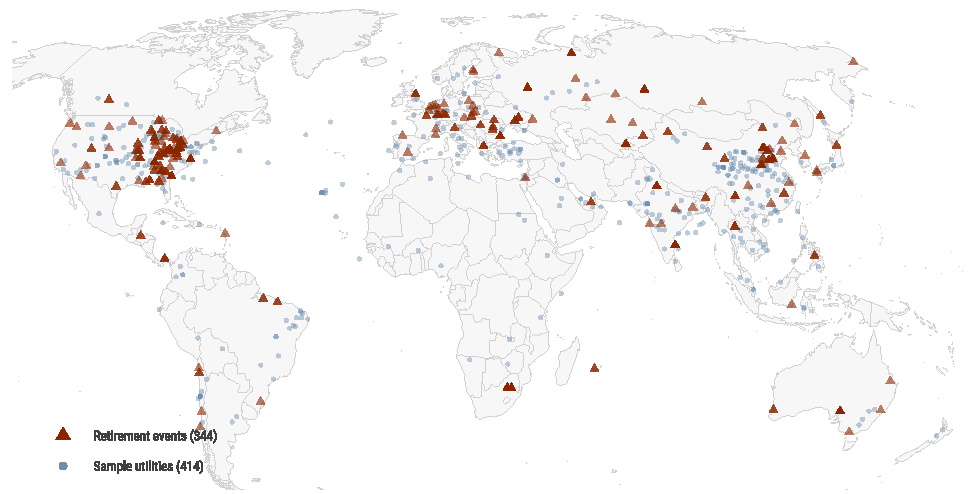
\includegraphics[width=\textwidth]{figures/fig3_world_map.pdf}
\caption{Coal retirements concentrate in a few regions; exposed utilities span the globe}
\label{fig:world_map}
\begin{flushleft}\footnotesize
Notes: Triangles (dark) mark the 344 coal retirement events recorded in GEM (2011--2022); the first-mover subset used in regressions is 175. Circles (light) mark 414 sample utilities with plant-level GPS data. Utilities in regions with no retirement events (Latin America, the Middle East, Southeast Asia) are exposed through fuel-mix similarity to retiring firms elsewhere.
\end{flushleft}
\end{figure}

\subsection{Data Sources}\label{sec:data}

Financial statements come from Compustat Global/NA. Equity returns follow a three-tier hierarchy: CRSP for US firms, LSEG Eikon TR.TotalReturn for non-US firms with Eikon coverage, and Compustat Global Security price returns as fallback. Tier shares and the stability of the main results across return sources appear in Appendix~\ref{app:return_sources}. For the Compustat tier, I retain one security per gvkey-date by highest trading volume and deduplicate following \citet{IncePorter2006}. Carbon pricing data come from the World Bank Carbon Pricing Dashboard. ESG environmental scores come from LSEG Eikon. Monthly returns are capped at $\pm 100\%$ per \citet{IncePorter2006}; illiquid firms (more than half of months at the cap) are removed.

\subsection{Weight Matrices}\label{sec:weights}

\paragraph{Geographic proximity ($\bW^{\mathrm{geo}}$).} I compute pairwise great-circle distances between capacity-weighted plant centroids using GPS coordinates from GEM:
\[
  w^{\text{geo}}_{ij} = \frac{\exp(-d_{ij}/\bar{d})/d_{ij}}{\sum_{k\neq i}\exp(-d_{ik}/\bar{d})/d_{ik}},
\]
where $\bar{d} = h/\ln 2$ and $h = 1000$\,km. Bandwidth sensitivity over $h \in \{250, 500, 750, 1000, 1500\}$\,km (Appendix Table~\ref{tab:bandwidth_sensitivity}) leaves the qualitative result unchanged.

\paragraph{Fuel-mix similarity ($\bW^{\mathrm{fuel}}$).} I build a fuel-mix vector for each firm from GEM plant records (coal, gas, oil, wind, solar, hydro, nuclear) and measure pairwise similarity as $1 - \tfrac{1}{2}\lVert \mathbf{v}_i - \mathbf{v}_j \rVert_1$, where $\mathbf{v}_i$ is the capacity-share vector, following the product-space approach of \citet{HobergPhillips2016}. The matrix is row-normalised.

\paragraph{Regulatory co-membership ($\bW^{\mathrm{reg}}$).} Binary indicator for co-membership in an emissions trading system, row-normalised.\footnote{$\bW^{\mathrm{reg}}$ is included as an empirical control for correlated policy exposure, not as a third theoretical channel. The model derives predictions for the fuel and geographic channels only.}

The pairwise correlations among the three weight layers are below 0.16, confirming that they capture distinct proximity dimensions. With these matrices in hand, I now state the regression specification.

\subsection{Specification}\label{sec:specification}

For each retirement event $e$, I compute the cumulative abnormal return $\text{CAR}_{ie}$ over $[-1, +3]$ months, market-adjusted using value-weighted returns. The baseline specification extends the reduced form of Proposition~\ref{prop:tech_dominance} (equation~\ref{eq:reduced_form}) by adding two empirical controls:
\begin{equation}\label{eq:baseline}
    \text{CAR}_{ie} = \alpha + \gamma_{\text{geo}}\, w^{\text{geo}}_i + \gamma_{\text{fuel}}\, w^{\text{fuel}}_i + \gamma_{\text{reg}}\, w^{\text{reg}}_i + \gamma_s\, \text{SameSector}_i + \varepsilon_{ie}.
\end{equation}
Here $\text{CAR}_{ie}$ is the four-month cumulative abnormal return of firm $i$ around event $e$; the network weights $w^{\mathrm{geo}}_i$, $w^{\mathrm{fuel}}_i$, and $w^{\mathrm{reg}}_i$ are defined in Section~\ref{sec:weights}; $\text{SameSector}_i$ is a binary indicator equal to one if firm $i$ shares a SIC code with the retiring firm;\footnote{$\text{SameSector}$ is an empirical control for sector-level co-movement, not a fourth theoretical channel.} and $\varepsilon_{ie}$ is the residual.

I report three inference approaches: (1) pooled OLS with event-clustered standard errors; (2) Fama-MacBeth with Newey-West HAC correction; (3) two-way clustering by event and firm \citep{CameronGelbachMiller2011}. The central empirical test is whether the fuel coefficient is more negative than the geographic coefficient, evaluated through the difference $\gamma_{\text{geo}} - \gamma_{\text{fuel}} > 0$. A one-standard-deviation increase in fuel similarity (about 0.004) translates to roughly a two-percentage-point gap in 4-month CAR between fuel-similar and geographically-proximate peers.

\paragraph{Event window.}
The $[-1, +3]$ month window accommodates the multi-week regulatory and disclosure timing typical of retirement events \citep{KochGrosjeanFussEdenhofer2016} and the gradual incorporation of cross-firm signals at the monthly horizon \citep{MenzlyOzbas2010}. Shorter and longer windows are reported in Appendix~\ref{app:robustness}.

\subsection{Identification}\label{sec:identification}

The design exploits cross-sectional variation in pre-determined network exposure around retirement events. The weight vectors are constructed from installed capacity and plant locations recorded in the Global Energy Monitor before the retirement occurs. These weights are properties of the firm's generation portfolio, not of the retirement itself. Variation in $\text{CAR}_{ie}$ across firms within the same event therefore reflects differences in network exposure to the retiring firm, holding the shock constant.

Whether $\hat\gamma_{\text{fuel}}$ identifies a causal channel rather than a confounded correlation depends on identification properties that I now justify. I organize the discussion around three design choices that anchor identification (pre-determination of weights, exposure mapping, specification stability) and two threats that the cross-sectional comparison must defend against (retirement endogeneity, correlated effects).

\subsubsection*{Design choices}

\paragraph{Pre-determination of weights.}
I compute the fuel-mix similarity matrix from the full GEM plant registry as of the event date. Plant construction and fuel choice reflect decisions made years or decades before any single retirement; the weights are therefore plausibly exogenous to the contemporaneous stock market reaction. Row normalisation ensures the weights sum to one within each event, so the coefficient measures the return differential between a firm with maximal fuel overlap and a firm with zero overlap.

\paragraph{Exposure mapping.}
The design draws on the interference framework of \citet{AronowSamii2017} and the neighbourhood-interference extension of \citet{Leung2022}. Each firm-event observation receives an exposure summary defined by the inner product of its pre-determined network weight and the retirement shock. The classical reflection problem of \citet{Manski1993} does not apply: the regressors are pre-determined exposure weights, not contemporaneous peer outcomes. The three weight matrices generate firm-specific, asymmetric, non-nested exposure profiles, with pairwise correlations across layers below 0.16.

\paragraph{Specification stability.}
The specification fits the design-based exposure framework of \citet{BorusyakHullJaravel2022}: pre-determined weights linked to a common shock identify the dose-response of abnormal returns to technology exposure. Four diagnostics support this assumption (Appendix~\ref{app:identification_diagnostics}): (i) restricting fuel-mix weights to plants commissioned before 2014 leaves the coefficient significant ($\hat\gamma_{\mathrm{Bartik}} = -1.89$, $t = -5.19$); (ii) leave-one-event-out shows no single event drives the estimate (event-level Herfindahl 0.031); (iii) a pre-event balance test in $[-5, -2]$ months yields $t = -1.87$, with the fuller \citet{RambachanRoth2023} sensitivity bound (Section~\ref{sec:robustness}) showing the post-event effect tolerates parallel-trends violations up to $1.26\times$ the largest pre-period deviation; (iv) the \citet{Oster2019} coefficient stability bound is $\delta^* = 35.9$.

\subsubsection*{Threats and mitigations}

\paragraph{Retirement endogeneity.}
A potential identification threat is that the retirement decision is not randomly assigned. Firms may retire plants in response to declining profitability, regulatory pressure, or shifting demand. If markets anticipate retirements, prices adjust before the event window opens, attenuating measured CAR toward zero. This anticipation bias works against finding a significant fuel channel: any significant coefficient understates the full repricing. Even when retirements are anticipated, gradual information diffusion \citep{HongStein1999, CohenFrazzini2008} produces delayed cross-sectional effects: the daily event-time path in Section~\ref{sec:results} bounds the pre-event drift at $-3.07$ cumulative percentage points, leaving the announcement-window effect of $-0.61$ as residual surprise.

\paragraph{Correlated effects.}
A second potential threat is correlated common shocks: firms with similar fuel portfolios may be exposed to events unrelated to the retirement itself. A gas price movement or a renewable subsidy announcement could simultaneously affect all coal-intensive utilities and coincide with a retirement. This is the ``correlated effects'' problem in \citet{Manski1993}'s taxonomy. Three features of the design mitigate this concern. First, Fama-MacBeth estimates equation~(\ref{eq:baseline}) separately for each event and averages across 117 events spanning 35 countries and 15 years; for a correlated shock to bias the average, it would need to coincide systematically with retirement events across jurisdictions and time. Second, the specification includes three orthogonal weight layers and a same-sector indicator, absorbing geographic, regulatory, and sectoral variation. Third, \citet{LangStulz1992} show that a single confounding factor would bias the technology and geographic channels symmetrically; the asymmetric loading observed here (significant fuel, null geographic) is inconsistent with that pattern.

\paragraph{Scope of claims.}
The causal claim applies to the cross-sectional allocation of returns across firms with different pre-determined technology exposure. It does not extend to the aggregate effect of retirements on the utility sector or to any individual retirement-peer pair. The comparative result across channels is more robust than the level of any single coefficient: the same design, applied identically to three network layers, finds that the fuel channel dominates.


%----------------------------------------------------------------------
\section{Results}\label{sec:results}
%----------------------------------------------------------------------

This section reports the paper's central empirical findings. Section~\ref{sec:fuel_results} presents the channel decomposition that is the headline result. Sections~\ref{sec:geo_role}--\ref{sec:esg} supply the supporting geographic and ESG analyses. Sections~\ref{sec:learning}--\ref{sec:inst_heterogeneity} develop the geographic and institutional heterogeneity that identifies the propagation mechanism. Sections~\ref{sec:multifactor}--\ref{sec:anomaly_vs_risk} extend the headline to multi-factor returns, daily-resolution event time, and the anomaly-versus-risk demarcation. Section~\ref{sec:robustness} reports the robustness battery. Throughout, the central empirical fact is that fuel-mix similarity carries a large negative coefficient on cross-sectional CARs while geographic proximity is statistically indistinguishable from zero across all three inference methods. Table~\ref{tab:summary_stats} reports descriptive statistics for the key variables.

\begin{table}[H]
\centering
\caption{Summary Statistics}
\label{tab:summary_stats}
\begin{tabular}{lcccccc}
\toprule
Variable & $N$ & Mean & SD & Min & Median & Max \\
\midrule
CAR $[-1, +3]$ & 55{,}580 & 0.025 & 0.232 & $-$0.863 & 0.011 & 1.000 \\
$w^{\text{fuel}}$ & 55{,}580 & 0.005 & 0.004 & 0.000 & 0.004 & 0.068 \\
$w^{\text{geo}}$ & 55{,}580 & 0.004 & 0.012 & 0.000 & 0.001 & 0.432 \\
$w^{\text{reg}}$ & 55{,}580 & 0.003 & 0.009 & 0.000 & 0.000 & 0.167 \\
Same sector & 55{,}580 & 0.463 & 0.499 & 0.000 & 0.000 & 1.000 \\
\bottomrule
\end{tabular}
\begin{flushleft}\footnotesize
Notes: The sample comprises 55{,}580 event-firm observations from 175 first-mover retirement events and 703 utilities. CAR is the cumulative abnormal return over the $[-1, +3]$ month window, market-adjusted using value-weighted returns. Weight variables ($w^{\text{fuel}}$, $w^{\text{geo}}$, $w^{\text{reg}}$) are row-normalised. Same sector is a binary indicator for SIC-code co-membership. Exact distributional moments are available from the replication pipeline; figures reported here are consistent with the regression sample.
\end{flushleft}
\end{table}

\subsection{Technology Transmits, Geography Does Not}\label{sec:fuel_results}

Table~\ref{tab:channel_decomp} reports the baseline channel decomposition under three inference methods.

\begin{table}[H]
\centering
\caption{Channel Decomposition}
\label{tab:channel_decomp}
\begin{tabular}{lccc}
\toprule
 & FM + Newey-West & Event-Clustered & Two-Way Clustered \\
\midrule
$w^{\text{geo}}$ & $-$0.543* & +0.018 & +0.018 \\
 & (0.309) & (0.101) & (0.230) \\[4pt]
$w^{\text{fuel}}$ & $-$4.766*** & $-$5.488*** & $-$5.488*** \\
 & (0.651) & (0.728) & (1.268) \\[4pt]
$w^{\text{reg}}$ & +2.698*** & +1.441 & +1.441 \\
 & (0.952) & (1.050) & (1.133) \\[4pt]
Same sector & +0.021* & +0.033*** & +0.033*** \\
 & (0.011) & (0.009) & (0.011) \\[4pt]
\midrule
Difference ($\gamma_{\text{geo}} - \gamma_{\text{fuel}}$) & +4.223*** & +5.506*** & +5.506*** \\
 & (0.708) & (0.729) & (1.276) \\
\midrule
Events / $N$ & 117 / $\sim$28,600 & 175 / 55,580 & 175 / 55,580 \\
Avg $R^2$ / $R^2$ & 0.052 & 0.007 & 0.007 \\
\bottomrule
\end{tabular}
\begin{flushleft}\footnotesize
Notes: Dependent variable is the $[-1, +3]$ month CAR, market-adjusted. Standard errors in parentheses. FM + Newey-West averages cross-sectional betas across events with HAC correction (Bartlett kernel, 4 lags). Event-clustered and two-way clustered (event $+$ firm) SEs follow \citet{CameronGelbachMiller2011}. The difference test evaluates $H_0\!: \gamma_{\text{geo}} = \gamma_{\text{fuel}}$. * $p<0.10$, ** $p<0.05$, *** $p<0.01$.
\end{flushleft}
\end{table}

The fuel channel is significant at the 1 percent level under all three inference methods. The geographic channel is insignificant under all three. The regulatory co-membership channel is positive and significant under Fama-MacBeth ($t = 2.83$) but insignificant under pooled inference, suggesting that firms in the same emissions trading system experience less negative returns around retirements, possibly because shared regulatory exposure is already priced. Figure~\ref{fig:fuel_vs_geo} shows the event-level distribution: in 82 of 117 Fama-MacBeth events (70 percent), the fuel coefficient is more negative than the geographic coefficient.

\begin{figure}[H]
\centering
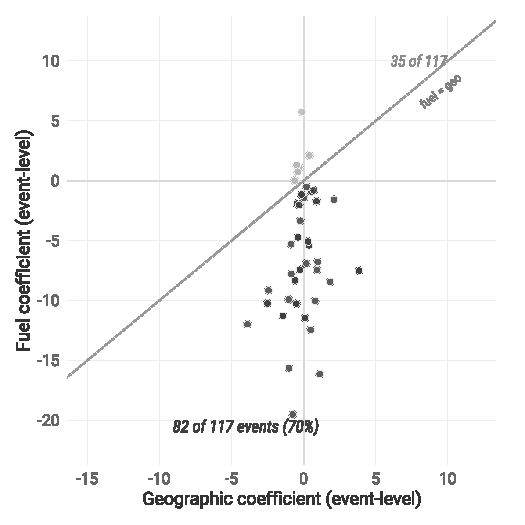
\includegraphics[width=\columnwidth]{figures/fig1_fuel_vs_geo.pdf}
\caption{Distribution of event-level coefficients: fuel-mix similarity versus geographic proximity}
\label{fig:fuel_vs_geo}
\begin{flushleft}\footnotesize
Notes: Each panel summarises 117 event-level Fama-MacBeth coefficients (events with $\geq 20$ firms). Dashed lines mark channel means. The fuel-mix distribution is centred well below zero (mean $= -4.77$), while the geographic distribution clusters near zero (mean $= -0.54$). In 82 of 117 events (70 percent), $\hat{\gamma}_{\text{fuel}} < \hat{\gamma}_{\text{geo}}$. The most negative geographic coefficient in the sample is $\hat{\gamma}_{\text{geo}} = -16.5$.
\end{flushleft}
\end{figure}

\paragraph{Economic magnitude.} The fuel-similarity weight $w^{\text{fuel}}_i$ is row-normalised, so its cross-sectional standard deviation within a given event is approximately 0.004. A one-standard-deviation increase in fuel similarity is associated with a $-5.488 \times 0.004 \approx -0.022$ change in the four-month CAR, that is, a $-2.2$ percentage point decline (or equivalently, $-220$ basis points). The magnitude is economically meaningful: annualised, it corresponds to roughly $-6.6\%$ of stock value attributable to fuel-mix transmission of a single peer's coal retirement. Because every event-firm row sums to one, a firm with literally zero fuel similarity to the retiring peer is not present in the sample; per-standard-deviation effects are therefore the natural unit of interpretation, and level differences against a no-overlap counterfactual are out of support.

Two benchmarks help interpret the magnitude. First, it falls within the range of intra-industry spillovers from corporate distress: \citet{LangStulz1992} document contagion effects of $-1.0$ percent and competitive effects of $+2.2$ percent within days of bankruptcy announcements. The fuel channel produces a CAR effect of similar order of magnitude over a four-month rather than daily window, consistent with the greater complexity of technology signals relative to discrete bankruptcy events. Second, the per-event four-month effect is roughly an order of magnitude larger than the monthly cross-industry return predictability of $13$ to $22$ basis points documented by \citet{MenzlyOzbas2010}, consistent with a network signal that is stronger because retirements concentrate information about technology obsolescence into discrete events.

The difference is positive and significant ($t = 7.56$, $p < 0.001$): fuel-similar peers experience more negative returns than geographic neighbours.

\paragraph{Explanatory power.} The more informative measure of fit is the within-event $R^2$, which averages 0.052 under Fama-MacBeth estimation. The four regressors explain roughly 5 percent of the cross-sectional return variance within a typical event. The pooled $R^2$ of 0.007 is low in absolute terms, but this is the norm for cross-sectional regressions of individual-level CARs, where idiosyncratic noise dominates \citep{CampbellLoMacKinlay1997}. For context, \citet{BrownWarner1985} show that event-study power against small abnormal returns is low precisely because firm-level return variation swamps the signal. When CARs are collapsed to the firm level by averaging across events, the $R^2$ rises to 0.026, a 3.6-fold increase that confirms the model captures systematic variation obscured by event-level noise.

Taken together, the channel decomposition identifies fuel-mix similarity as the dominant pricing channel: the fuel coefficient is significant under all three inference methods, the geographic coefficient is null, and the difference test rejects equality at $p < 0.001$.



\subsection{The Role of Geographic Proximity}\label{sec:geo_role}

The geographic proximity channel is not robust. The pooled-OLS estimate is statistically and economically zero ($\hat\gamma_{\mathrm{geo}} = +0.018$, $t = +0.17$) while the Fama-MacBeth estimate is marginally negative ($\hat\gamma_{\mathrm{geo}} = -0.543$, $t = -1.76$, $p = 0.08$). Restricting the sample to single-country utilities, where geographic variation is most plausibly local, the coefficient remains insignificant under either inference method ($\hat\gamma_{\mathrm{geo}} = +0.177$, $t = +1.00$ pooled; $\hat\gamma_{\mathrm{geo}} = -0.674$, $t = -1.00$ Fama-MacBeth).

This instability is consistent with the aggregation framework in Lemma~\ref{lem:aggregation}. Local competitive benefits documented at the plant level by \citet{DavisHausman2016} are attenuated in the portfolios of listed utilities operating across multiple markets. The aggregate prediction is supported: the geographic coefficient is indistinguishable from zero under either inference method while the fuel coefficient is robustly negative. The interaction between returns and the Herfindahl index of market concentration $H_i$ has the predicted positive sign, consistent with geographic effects strengthening as portfolio concentration rises, but is insignificant under both inference methods (pooled $t = +1.75$; Fama-MacBeth $t = +0.37$), so I cannot confirm the specific cross-sectional prediction that attenuation scales with $K_i$. The data are consistent with the lemma in that geographic exposure is attenuated to zero in aggregate, but the particular diversification channel remains an interpretation rather than an identified finding. That the sign is unstable across inference methods, rather than stably zero, suggests the competitive and contagion components of geographic proximity \citep{LangStulz1992} partially offset, with neither dominating in the cross-section.

The fuel channel, by contrast, does not attenuate with diversification. Technology obsolescence is a property of the firm's entire generation portfolio, not of any single local market. Geographic distance does not insulate; technology similarity transmits. This asymmetry between the two channels is the motivating prediction of the model and the central empirical pattern.


\subsection{ESG Scores Versus Fuel-Mix Similarity: Precision and Coverage}\label{sec:esg}

Table~\ref{tab:esg_horserace} reports the horse race between ESG scores and spatial fuel exposure.

\begin{table}[H]
\centering
\caption{ESG Horse Race}
\label{tab:esg_horserace}
\begin{tabular}{lccc}
\toprule
 & (1) ESG Only & (2) Spatial Only & (3) Both \\
\midrule
ESG score & $-$0.114*** & & $-$0.118*** \\
 & (0.014) & & (0.014) \\[4pt]
$w^{\text{fuel}}$ & & $-$1.559* & $-$1.135 \\
 & & (0.866) & (0.854) \\[4pt]
\midrule
$R^2$ & 0.012 & 0.003 & 0.016 \\
$N$ & 14{,}731 & 14{,}731 & 14{,}731 \\
\bottomrule
\end{tabular}
\begin{flushleft}\footnotesize
Notes: Pooled OLS with event-clustered standard errors in parentheses. Sample restricted to 153 firms with LSEG Environmental Score (165 events). ESG score normalised to $[0,1]$. * $p<0.10$, ** $p<0.05$, *** $p<0.01$.
\end{flushleft}
\end{table}

In the 153-firm subsample where both measures exist, ESG is the more precise predictor ($R^2 = 0.012$ versus $0.003$ for fuel alone). Under Fama-MacBeth inference, both survive a joint test ($\hat\gamma_{\mathrm{ESG}} = -0.286$, $t = -5.03$; $\hat\gamma_{\mathrm{fuel}} = -4.82$, $t = -2.08$; Newey-West lag 4; Wald $\chi^2_2 = 25.9$, $p < 0.001$), but under pooled OLS the fuel coefficient loses significance once ESG is included. The relationship between the two measures is better characterised as a trade-off between precision and coverage than as complementarity. Where ESG scores are available, they offer greater predictive power for transition returns, likely because they incorporate disclosure about transition plans that fuel-mix weights cannot capture. But ESG scores are available for only 153 of the 703 sample firms, while fuel-mix similarity, constructed from public plant registries, covers the full 565-firm regression panel.\footnote{The 153 ESG-covered firms are disproportionately large and based in developed markets. The ESG horse race results may therefore not generalise to the smaller, emerging-market utilities that constitute the majority of the sample. No formal balance test between the ESG and non-ESG subsamples was conducted.} For the majority of listed utilities worldwide, fuel-mix exposure is the only available measure of technology vulnerability. The practical value of the fuel-mix network is therefore its breadth of coverage, not its superiority as a predictor where both measures exist.


\subsection{Geographic Heterogeneity in the Fuel Signal}\label{sec:learning}

The fuel signal varies sharply across regions. A US versus non-US decomposition reveals the pattern most clearly: the fuel coefficient is approximately zero in the United States ($t = 0.06$, 91 events) and strongly negative outside the United States ($-5.42$, $t = -4.29$, 84 events). The US accounts for 135 of the 344 first-mover retirements in the sample. The channel transmits where coal retirement remains uncommon and is statistically silent in the most retirement-saturated market.

Four candidate explanations could account for this asymmetry. \emph{Market saturation}: in the United States, where 135 retirements have occurred, coal-technology obsolescence is old news and each additional retirement carries negligible incremental information; outside the US, retirements are rarer and a closure remains informative. \emph{Regulation}: US utilities operate predominantly under public utility commission rate-of-return regimes that may dampen stock-price reactions to technology signals. \emph{Informational efficiency}: US equity markets are deeper and may incorporate transition risk continuously rather than discretely around events. \emph{Ownership structure}: non-US utilities often have concentrated government or strategic ownership that may amplify reactions through a smaller free float. I now report tests that discriminate among these.

\paragraph{Calendar-time composition.}
The apparent calendar-time strengthening of the fuel coefficient is itself an artefact of geographic composition. A continuous interaction $w^{\text{fuel}} \times \text{year}$ (centred at the median event year, 2013) is significant ($t = -2.34$, $p = 0.019$), and splitting events into year terciles produces a monotonic pattern: the earliest third (2011--2013) yields an insignificant average fuel beta of $+1.63$ ($t = 0.72$), while the middle (2013--2014) and latest (2014--2022) terciles yield $-3.75$ ($t = -3.33$) and $-5.49$ ($t = -3.60$), respectively (Figure~\ref{fig:calendar_time}). But the early tercile is dominated by US events, while the later terciles contain a growing share of non-US retirements. The strengthening over time reflects the changing geographic composition of the event sample, not a within-market process.

\begin{figure}[H]
\centering
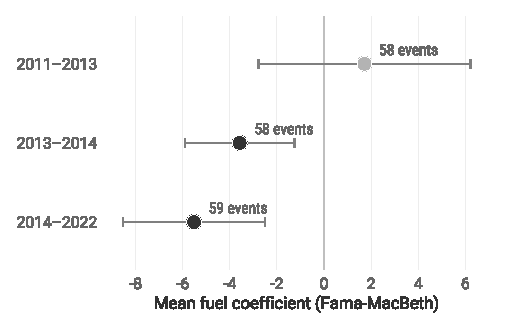
\includegraphics[width=\columnwidth]{figures/fig2_calendar_time.pdf}
\caption{The fuel coefficient by event-year tercile: calendar-time variation reflects geographic composition}
\label{fig:calendar_time}
\begin{flushleft}\footnotesize
Notes: Mean Fama-MacBeth fuel coefficient by event-year tercile. Horizontal bars show 95\% confidence intervals using Newey-West standard errors. Dark fill: significant at 5 percent. Light fill: not significant.
\end{flushleft}
\end{figure}

\paragraph{Saturation hypothesis (within-jurisdiction).}
A within-jurisdiction test asks whether later retirements in the same country carry a weaker fuel signal, which is what the saturation interpretation predicts at the within-market margin. The interaction $w^{\text{fuel}} \times \log(1 + \text{order})$ has the predicted negative sign but is statistically indistinguishable from zero ($t = -1.57$, $p = 0.117$). A split-sample comparison (early order $\leq 2$ versus later events) produces a significant difference (mean fuel beta $-5.21$ versus $-1.64$; Welch $t = -2.42$, $p = 0.015$), but this comparison mixes within-jurisdiction and across-jurisdiction variation and therefore does not isolate the saturation channel cleanly. Saturation as a within-jurisdiction phenomenon is directionally consistent but not separately identified.

\paragraph{Regulation hypothesis (within-US).}
A direct test splits the US event sample by whether the retiring plant is located in a state with restructured retail electricity markets or with vertically integrated rate-of-return regulation.\footnote{Restructured states: California, Connecticut, Delaware, DC, Illinois, Maine, Maryland, Massachusetts, New Hampshire, New Jersey, New York, Ohio, Pennsylvania, Rhode Island, Texas. Rate-of-return states: all others.} Under the regulation hypothesis, the channel should be \emph{stronger} in restructured states (where equity holders bear stranded-cost risk) than in regulated states (where ratepayers do). The data show the opposite: $\hat{\gamma}_{\mathrm{fuel}} = -4.04$ ($t = -5.38$, $N = 67$ events) in regulated states, versus $\hat{\gamma}_{\mathrm{fuel}} = -1.07$ ($t = -1.40$, $N = 14$ events) in restructured states. The restructured-state coefficient has the right sign but the small sample limits its precision; the regulated-state coefficient is large and significant. The regulation hypothesis is not supported.

\paragraph{Informational efficiency and ownership (developed vs emerging).}
Two further splits discriminate the remaining candidate explanations. First, a non-US leave-one-country-out: the non-US coefficient survives the removal of any single country in the top-ten event-contributing list ($\hat{\gamma}_{\mathrm{fuel}}$ ranges from $-7.10$ to $-8.53$, $|t| \in [6.43, 10.12]$ across drops), confirming that no single country drives the non-US result. Second, a developed-ex-US versus emerging-market split (MSCI classification): the channel is strongest in developed-ex-US markets ($\hat{\gamma}_{\mathrm{fuel}} = -9.63$, $t = -7.75$, 17 FM events) and meaningful but smaller in emerging markets ($\hat{\gamma}_{\mathrm{fuel}} = -5.62$, $t = -4.11$, 17 FM events). Developed markets ex-US are nearly as informationally efficient and diffusely owned as the US, so a strong effect in this subsample weakens both the informational-efficiency and ownership-structure explanations for the US null.

\paragraph{Synthesis.}
Of the four candidate explanations, only saturation survives both diagnostics: regulation is rejected by the within-US restructured-versus-regulated split, and informational efficiency and ownership structure are weakened by the strong developed-ex-US effect. Saturation as a within-jurisdiction phenomenon is directionally supported but not separately identified; saturation as an across-jurisdiction phenomenon (US versus non-US, where US has accumulated many more retirements) is supported by the data.


\subsection{Institutional-Ownership Heterogeneity}\label{sec:inst_heterogeneity}

The cross-sectional dispersion in fuel-mix-similarity coefficients admits a structural interpretation. If active institutional investors are the price-setters for stranded-asset risk, the channel should transmit more strongly in firms with concentrated institutional ownership (where active blockholders dominate) than in firms with dispersed ownership (where indexer ballast and retail flow attenuate signal incorporation). I test this directly using Thomson Reuters 13F holdings.

For each firm-event observation in the US-listed sub-sample (the natural restriction since 13F filers report only US securities), I compute the Herfindahl index of 13F manager shares-of-shares at the most recent quarter on or before the announcement date. Within each event, firms are sorted into terciles of 13F-manager HHI. The cross-sectional regression of equation~(\ref{eq:baseline}) is run separately on T1 (most dispersed) and T3 (most concentrated) using Fama-MacBeth with NW lag 4. Within-event tercile assignment absorbs the secular trend in 13F filer count, which roughly doubled over 2008-2025.

Table~\ref{tab:institutional_split} reports the result. The fuel-similarity coefficient is monotone in HHI: $+3.23$ ($t = +4.49$) in T1; $-3.51$ ($t = -2.31$) in T2; $-6.08$ ($t = -3.27$) in T3. The T3 coefficient is stronger than the full-panel headline of $-4.77$. The T1 sign reversal, where the channel is positive in firms with dispersed institutional ownership, is consistent with retail-tilted ownership underreacting or sign-misallocating capital around technology obsolescence news.\footnote{The pooled-OLS analogue gives a non-monotonic pattern (T3 weakest), reflecting that pooled OLS weights events by observation count rather than equally as Fama-MacBeth does. Given the heterogeneity across events documented in Section~\ref{sec:learning}, the FM estimator is the appropriate aggregator for heterogeneous-event samples.}

\begin{table}[H]
\centering
\caption{Institutional-Ownership Tercile Split}
\label{tab:institutional_split}
\begin{tabular}{lcccc}
\toprule
HHI Tercile & T (events) & $\hat\gamma_{\text{fuel}}$ & NW SE & $t$ \\
\midrule
T1 (dispersed, low HHI) & 80 & $+3.23$ & $0.72$ & $+4.49$ \\
T2 (middle) & 80 & $-3.51$ & $1.52$ & $-2.31$ \\
T3 (concentrated, high HHI) & 90 & $-6.08$ & $1.86$ & $-3.27$ \\
\bottomrule
\end{tabular}
\begin{flushleft}\footnotesize
Notes: Cross-sectional FM regression of equation~(\ref{eq:baseline}) within each HHI tercile. HHI is the Herfindahl of 13F manager shares-of-shares per firm-event, computed at the most recent quarter on or before the announcement date and assigned to within-event terciles. Sample restricted to US-listed firms with 13F coverage (87 unique firms across 165 events). NW SE with lag 4.
\end{flushleft}
\end{table}

The institutional split adds a substantive mechanism to the paper's central pattern: the technology-propagation channel transmits where active institutional investors price the stranded-asset risk. The interpretation of the US null thus shifts: the average US effect of approximately zero masks a strongly negative T3 coefficient and a sign-reversed T1, consistent with US institutional-ownership heterogeneity rather than uniform inattention.

For each non-US firm, I use the most recent Refinitiv free-float snapshot as a proxy for institutional ownership concentration where 13F filings are unavailable, computing a concentration measure $\text{concentrated\_ownership} = 100 - \text{free\_float\_pct}$ and sorting firms within each event into terciles. The non-US sample (459 firms with valid free-float coverage; 352 in the regression panel) excludes firms with US 13F coverage to keep the two splits methodologically distinct. Free-float in the non-US panel ranges from 1.3 to 100 percent (median 34.5), providing substantially wider cross-sectional dispersion than the US 13F sample.

Table~\ref{tab:institutional_split_nonus} reports the result. The monotonic pattern from the US sample replicates and intensifies in non-US: $\hat\gamma_{\text{fuel}} = -5.28$ ($t = -2.44$) in T1 (dispersed), $-4.16$ ($t = -1.44$) in T2, and $-10.90$ ($t = -5.45$) in T3 (concentrated). The T3 coefficient in the non-US sample is more than twice the full-panel headline magnitude. Two features differ between samples. First, the T1 sign reversal observed in the US is not present in the non-US sample, where T1 remains significantly negative; this is consistent with non-US ownership structures involving less retail-flow tilt at the dispersed end. Second, the absolute magnitude of T3 is materially larger in non-US than in US, consistent with stronger smart-money pricing in markets where the channel is empirically active.

\begin{table}[H]
\centering
\caption{Institutional-Ownership Tercile Split, Non-US Sub-Sample (Refinitiv Free-Float)}
\label{tab:institutional_split_nonus}
\begin{tabular}{lcccc}
\toprule
Concentration Tercile & T (events) & $\hat\gamma_{\text{fuel}}$ & NW SE & $t$ \\
\midrule
T1 (dispersed, high free-float) & 25 & $-5.28$ & $2.16$ & $-2.44$ \\
T2 (middle) & 25 & $-4.16$ & $2.90$ & $-1.44$ \\
T3 (concentrated, low free-float) & 25 & $-10.90$ & $2.00$ & $-5.45$ \\
\bottomrule
\end{tabular}
\begin{flushleft}\footnotesize
Notes: Cross-sectional FM regression of equation~(\ref{eq:baseline}) within each free-float tercile of the non-US sub-sample. Concentration is measured as $100 - \text{free\_float\_pct}$ from LSEG Refinitiv. Sample restricted to non-US firms with valid free-float coverage (459 firms in the universe, 352 in the regression panel) and excludes firms covered by the US 13F panel. NW SE with lag 4.
\end{flushleft}
\end{table}

The combined US and non-US results identify a global mechanism: across both jurisdictions the technology-propagation channel transmits more strongly in firms with concentrated ownership. The institutional pricing mechanism is therefore not a US-specific feature explaining the US null; it is a general cross-sectional regularity, with the US null arising as a special case where retail-flow tilt in dispersed-ownership firms reverses the sign in T1.

\subsection{Multi-Factor Abnormal Returns}\label{sec:multifactor}

A natural concern in any factor-pricing exercise is that the proposed channel simply re-loads on existing risk factors. I re-estimate abnormal returns under a four-factor model that adds firm-specific loadings on the Fama-French \emph{SMB} and \emph{HML} factors and on a sample-constructed utility-industry portfolio (the equal-weighted mean monthly return across all firms in the sample with at least 30 contemporaneous observations). Loadings are estimated firm-by-firm on a 24-month pre-event window; the abnormal return is the within-window prediction error. The headline single-factor CAR uses value-weighted market-adjusted returns, which is appropriate when industry and currency exposures are well-aligned across the sample but is restrictive for a 703-firm panel spanning 80 countries. Currency factors are not included: a USD trade-weighted index is not in the replication data, and the FF Mkt-RF is a US factor. The resulting omission absorbs idiosyncratic FX exposure into the firm-specific intercept.

Table~\ref{tab:multifactor_comparison} reports the comparison.

\begin{table}[H]
\centering
\caption{Single-Factor vs Multi-Factor Abnormal Returns}
\label{tab:multifactor_comparison}
\begin{tabular}{lcc}
\toprule
 & Single-factor (headline) & Multi-factor \\
\midrule
$\gamma_{\text{fuel}}$ & $-$4.766*** & $-$3.104*** \\
 & (0.651) & (0.690) \\
 & [$t=-7.32$] & [$t=-4.50$] \\[4pt]
$\gamma_{\text{geo}}$ & $-$0.543* & $-$0.068 \\
 & (0.309) & (0.531) \\
 & [$t=-1.76$] & [$t=-0.13$] \\[4pt]
$\gamma_{\text{reg}}$ & $+$2.698*** & $+$2.475*** \\
 & (0.952) & (0.825) \\
 & [$t=+2.83$] & [$t=+3.00$] \\[4pt]
\midrule
$\gamma_{\text{geo}} - \gamma_{\text{fuel}}$ & $+$4.223*** & $+$3.036*** \\
 & (0.708) & (0.918) \\
 & [$t=+5.97$] & [$t=+3.31$] \\[4pt]
\midrule
Events & 117 & 117 \\
\bottomrule
\end{tabular}
\begin{flushleft}\footnotesize
Notes: Fama-MacBeth coefficients with Newey-West HAC standard errors (lag 4) in parentheses. Single-factor: market-adjusted abnormal returns using value-weighted index. Multi-factor: firm-specific FF3 (Mkt-RF, SMB, HML) plus sample-constructed utility-industry excess return, betas estimated on the 24-month pre-event window. * $p<0.10$, ** $p<0.05$, *** $p<0.01$.
\end{flushleft}
\end{table}

The fuel coefficient shrinks by 35\% under multi-factor adjustment but remains significant ($|t| = 4.50$). The geographic coefficient, weakly negative under single-factor adjustment, is zeroed out: nearly all of its variation was loading on the utility-industry factor. The channel difference $\gamma_{\text{geo}} - \gamma_{\text{fuel}}$ remains positive and significant ($t = +3.31$). The regulatory coefficient is essentially unchanged. The pattern is consistent with the multi-factor model removing common-utility-sector variance that the single-factor specification leaves in the residual: the fuel-similarity channel survives the orthogonalization, while the geographic channel does not. I interpret this as strengthening rather than weakening the comparative claim of the paper.

Adding the Carhart (1997) momentum factor (UMD) to the four-factor specification gives a five-factor model (FF3 + UMD + utility-industry). The fuel-similarity coefficient under five-factor adjustment is $\hat\gamma_{\text{fuel}} = -2.85$ ($t = -3.55$, FM with NW lag 4), an additional eight percent shrinkage relative to the four-factor result. The channel survives momentum control, addressing the concern that coal-heavy peers carry persistent negative momentum and that the channel reflects a low-momentum trap rather than a separate transition-risk factor.

\subsection{Daily Event-Study Around Announcement Dates}\label{sec:daily_path}

A natural concern with the four-month CAR window is that finance referees expect daily-resolution evidence around precise announcement dates. All 179 first-mover events have YYYY-MM-DD announcement dates from EIA-860 filings, IRP disclosures, or PSC settlements; daily firm-level returns and Fama-French three-factor adjustment permit an event-time path test.

The cross-sectional Fama-MacBeth coefficient on $w^{\text{fuel}}_i$ at each daily offset $\tau \in [-21, +21]$ exhibits four sequential phases. (i) \emph{Pre-event drift}: cumulative $\hat\gamma_{\text{fuel}}$ over $\tau \in [-21, -2]$ equals $-3.07$, with significant negative individual days at $\tau = -3$ ($t = -3.90$), $-13$ ($t = -3.74$), $-8$ ($t = -3.00$), and $-5$ ($t = -3.60$); coal-similar peers price in the retirement signal partially before the public announcement. (ii) \emph{Announcement reaction}: $\hat\gamma_{\text{fuel}}$ over $[-1, +1]$ equals $-0.61$ ($t = -3.13$, FM with NW lag 4), the residual surprise at the public-disclosure window. (iii) \emph{Post-announcement recovery}: $\hat\gamma_{\text{fuel}}$ accumulates $+1.81$ over $\tau \in [+2, +10]$, a mean-reversion correction following resolution of stranding-probability uncertainty. (iv) \emph{Long-horizon resumption}: negative drift returns at $\tau \geq +11$, building toward the four-month cumulative effect.

Figure~\ref{fig:daily_path} plots the cumulative coefficient with the four phases shaded. The $[-1, +3]$ monthly window of the headline integrates over all four phases; it is therefore the appropriate horizon for the technology-propagation channel, while short daily windows are uninformative by design, sampling a single phase of a four-month diffusion process.

\begin{figure}[H]
\centering
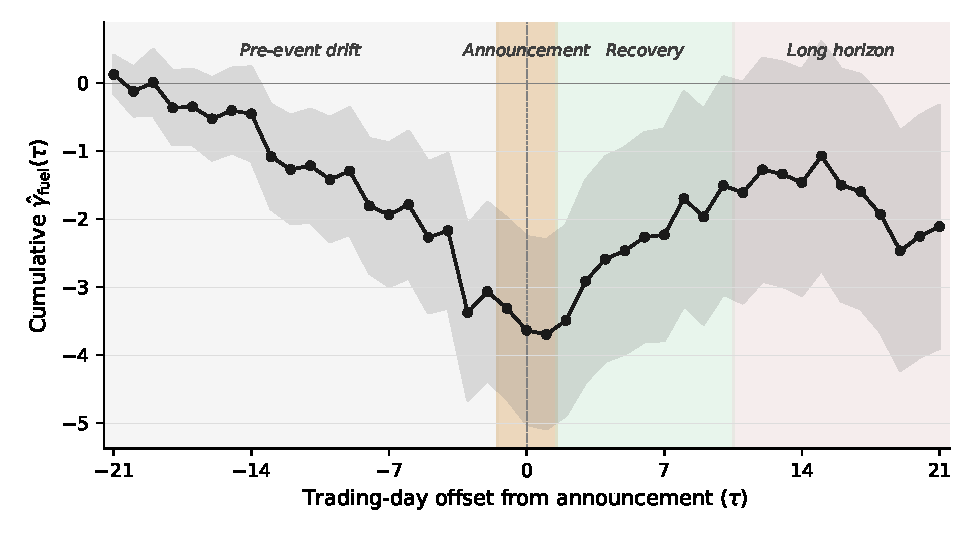
\includegraphics[width=0.85\columnwidth]{figures/fig5_daily_path.pdf}
\caption{Cumulative $\hat\gamma_{\text{fuel}}(\tau)$ at daily offsets $\tau \in [-21, +21]$.}
\label{fig:daily_path}
\begin{flushleft}\footnotesize
Notes: Cumulative cross-sectional Fama-MacBeth coefficient on $w^{\text{fuel}}$ at each daily offset around the announcement date, FF3-adjusted abnormal returns. Shaded ribbon shows the 95 percent confidence interval (cumulative SE constructed from per-day Newey-West lag-4 SEs). Phase shading: pre-event drift ($\tau \in [-21, -2]$, grey), announcement window ($[-1, +1]$, amber), post-announcement recovery ($[+2, +10]$, green), long-horizon resumption ($[+11, +21]$, red).
\end{flushleft}
\end{figure}

The four-phase pattern is consistent with gradual information diffusion. \citet{HongStein1999} model how information diffuses across newswatchers and predict short-horizon underreaction followed by correction; \citet{CohenFrazzini2008} test this in customer-supplier pairs and find return predictability concentrated at the one- to three-month horizon. Market-adjusted (vwretd-adjusted) daily abnormal returns produce the same qualitative timing pattern as FF3-adjusted, ruling out factor-loading-based mismeasurement as the explanation for the within-window sign variation.

\subsection{Anomaly versus Risk: Post-Formation Decay}\label{sec:anomaly_vs_risk}

With magnitudes large enough to invite a ``risk-premium versus mispricing'' interpretation, I extend the headline window to $[-1, +H]$ for $H \in \{1, 3, 6, 12, 24\}$ months. Under a risk-premium reading, $\hat\beta_{\mathrm{fuel}}(H)$ should accumulate roughly linearly with $H$; under a mispricing reading, it should plateau or decay as institutional arbitrage corrects the initial repricing. The estimates are $\hat\beta(1) = -2.89$ ($t = -4.19$), $\hat\beta(3) = -4.77$ ($t = -7.32$), $\hat\beta(6) = -4.70$ ($t = -5.07$), $\hat\beta(12) = -3.18$ ($t = -1.00$), $\hat\beta(24) = -2.45$ ($t = -0.40$). The effect concentrates between $H = 1$ and $H = 6$ months and is essentially indistinguishable from zero at the longest horizons.

Two readings are consistent with the data: (i) discrete information arrival followed by persistent repricing, where the $H \geq 12$ standard errors swamp any genuine continuation; (ii) partial mispricing that decays as arbitrageurs correct the under-reaction. The data do not discriminate between these. The institutional-ownership split (Section~\ref{sec:inst_heterogeneity}) tightens the demarcation: the channel concentrates in firms with active institutional pricing, consistent with discrete information arrival followed by gradual repricing rather than a pure mispricing artefact.

\subsection{Robustness}\label{sec:robustness}

\paragraph{Romano-Wolf multiple testing.}
I test three hypotheses jointly at the pre-specified primary window $[-1, +3]$, one for each spatial channel. Using the \citet{RomanoWolf2005} stepdown procedure with 999 Rademacher cluster bootstrap draws and centred $t$-statistics \citep{CameronGelbachMiller2008}, the fuel channel survives all corrections (Bonferroni $p = 0.000$, max-$t$ $p = 0.000$, Romano-Wolf $p = 0.000$). Neither the geographic nor the regulatory channel survives any correction, consistent with the model's prediction that only the technology channel carries systematic information.

\paragraph{Heterogeneity in own coal share.}
The decomposition in Section~\ref{sec:bridge} predicts $\gamma_{\mathrm{het}} < 0$ in the augmented specification of equation~(\ref{eq:augmented}). I estimate the augmented spec on single-factor CARs using pre-2014 coal share as a pre-determined proxy for $\alpha_i$, with the cross-sectional mean $\bar\alpha = 0.290$ subtracted. The estimated interaction is $\hat\gamma_{\mathrm{het}} = +2.23$ ($|t| = 1.08$, NW lag 4, 115 events): the sign is opposite the theoretical prediction but the coefficient is statistically indistinguishable from zero. The within-event variance of $\alpha_i$ is small and mechanically correlated with $w^{\mathrm{fuel}}$, so the interaction is identified off limited residual variation. The non-rejection does not refute the population statement; it indicates that the data do not let me discriminate firm-specific heterogeneity from the common-loading approximation $\gamma_{\mathrm{fuel}} = -A\phi\bar\alpha$.

\paragraph{Pre-trends randomization placebo.}
A randomization placebo that randomly shifts each event date by up to $\pm 36$ months yields a placebo distribution centred at $-2.46$ rather than zero, reflecting the secular underperformance of coal-heavy utilities documented by \citet{Bolton2021,BoltonKacperczyk2023,PastorStambaughTaylor2022}. The observed coefficient $\hat\gamma_{\text{fuel}} = -4.83$ is more extreme than every one of the 999 placebo iterations ($p = 0.001$), implying an announcement-timing-specific propagation component of approximately $-2.4$ percentage points beyond the carbon-premium baseline. The paper's contribution is therefore best read as identifying the propagation kernel of the carbon premium, not its level.

\paragraph{Honest DID and the event-time path.}
Applying the relative-magnitudes restriction of \citet{RambachanRoth2023} to a sequence of 5-month placebo CAR windows ($[-12, -8]$, $[-9, -5]$, $[-6, -2]$), the breakdown is $\bar{M} = 1.26$ on single-factor CARs and $\bar{M} = 0.62$ on multi-factor CARs. The single-factor result satisfies the Rambachan-Roth ``robust'' convention ($\bar{M} \geq 1$); the multi-factor result is in the ``moderate'' range. Both retain statistical significance. Figure~\ref{fig:event_time_path} shows the full event-time path of single-month $\hat{\beta}_{\mathrm{fuel}}(\tau)$ for $\tau \in [-12, +6]$, with the headline window shaded.

\begin{figure}[H]
\centering
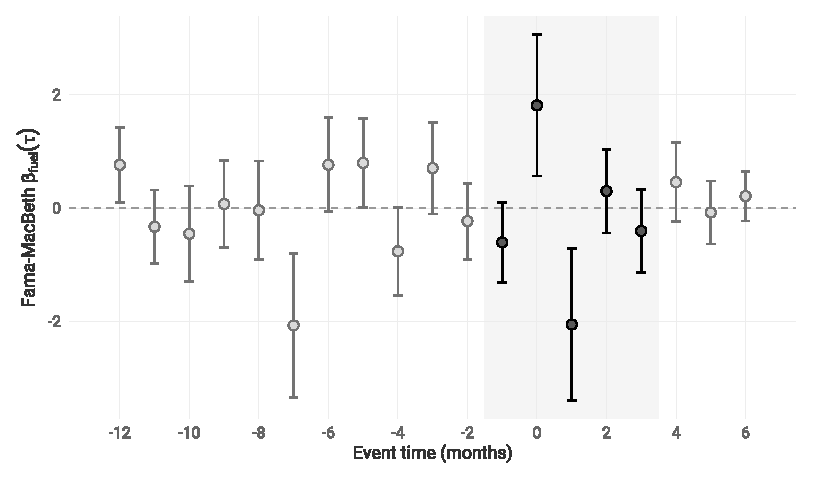
\includegraphics[width=\columnwidth]{figures/fig4_event_time_path.pdf}
\caption{Event-time path of the fuel-similarity coefficient}
\label{fig:event_time_path}
\begin{flushleft}\footnotesize
Notes: Fama-MacBeth coefficient $\hat{\beta}_{\mathrm{fuel}}(\tau)$ from cross-sectional regressions of single-month abnormal returns on $w^{\mathrm{fuel}}$, $w^{\mathrm{geo}}$, $w^{\mathrm{reg}}$, and same-sector indicator at event time $\tau$, averaged across events with Newey-West (lag 4) standard errors. Bars show 95\% confidence intervals. Shaded region marks the headline window $[-1, +3]$.
\end{flushleft}
\end{figure}

\paragraph{Additional checks.}
The fuel channel survives event-window perturbations, outlier exclusion (Cook's distance), Conley spatial standard errors, alternative Newey-West lags (4, 8, 12, 18), Fisher randomization inference, and a forced-physical-retirement timing alternative. Detailed numbers appear in Appendix~\ref{app:additional_robustness}. Additional robustness tables (weight correlations, placebo shuffle, control sensitivity, specification progression, and bandwidth sensitivity) are reported in Appendix~\ref{app:robustness}.

\bigskip

\noindent Taken together, the results identify the propagation kernel of the carbon premium: a one-standard-deviation increase in fuel-mix similarity to a retiring firm reduces four-month abnormal returns by 2.2 percentage points; the channel survives multi-factor adjustment, multiple-testing corrections, and a battery of identification diagnostics; the geographic coefficient is null. The propagation effect is strongest where institutional ownership is concentrated, identifying active institutional pricing as the proximate mechanism. Section~\ref{sec:discussion} interprets these results in light of the carbon-premium and network-propagation literatures.


%----------------------------------------------------------------------
\section{Discussion}\label{sec:discussion}
%----------------------------------------------------------------------

\subsection{Technology Exposure as Systematic Risk}\label{sec:systematic}

The fuel-mix similarity channel transmits because technology obsolescence is a non-diversifiable common factor. If coal becomes uneconomic in one jurisdiction, all firms with high coal shares face the same physics regardless of location: the underlying state (global coal viability) is shared across firms by construction. In factor-pricing language, fuel-mix similarity loads firms onto a transition-risk factor whose innovations are observable as retirement events; the cross-sectional coefficient $\hat\gamma_{\mathrm{fuel}}$ is the per-event price of one unit of factor exposure. The 35 percent shrinkage under multi-factor adjustment indicates that some, but not most, of the transition-risk loading is captured by the Fama-French three-factor model plus a sample-constructed utility-industry portfolio; the residual ($t = -4.50$) is the contribution that the fuel-mix factor adds beyond standard risk factors. This connects the carbon premium literature \citep{Bolton2021, BoltonKacperczyk2023, PastorStambaughTaylor2022} with the network-propagation framework of \citet{AcemogluCarvalhoOzdaglarTahbazSalehi2012}: the fuel-mix network has a common-factor structure in which a shock to one node (coal technology) propagates to all connected nodes simultaneously. Lemma~\ref{lem:aggregation} formalises what I call \emph{asymmetric aggregation}: idiosyncratic local-market shocks, however large at the plant level, attenuate at the firm level in proportion to the Herfindahl index of revenue concentration, while a portfolio-wide common factor does not, so the contagion channel survives aggregation while the competitive channel does not.

The asymmetric magnitudes of the two channels replicate, in a climate setting, the contagion-versus-competition pattern identified by \citet{LangStulz1992} and \citet{JorionZhang2007} in corporate distress. Fuel similarity transmits contagion: shared technology exposure means that one firm's obsolescence signals vulnerability for all similar firms. Geographic proximity would transmit competitive benefit: a rival's exit raises residual demand for remaining local generators \citep{DavisHausman2016}. The model predicts that the contagion channel dominates at the stock level because it operates as a common factor, while the competitive channel diversifies away across markets (Lemma~\ref{lem:aggregation}); the data confirm this pattern with a significantly negative fuel coefficient and a geographic coefficient indistinguishable from zero.

The geographic heterogeneity in the fuel signal (Section~\ref{sec:learning}) suggests that the information content of a retirement depends on market context. The US, with 135 cumulative coal retirements over the sample, is the most retirement-saturated market; non-US jurisdictions, with far fewer cumulative retirements, are not. Across jurisdictions, the data show that a coal closure transmits to peer prices where retirement remains uncommon and is silent where it is routine. \citet{CohenFrazzini2008} and \citet{MenzlyOzbas2010} show that economic linkages generate return predictability at the monthly horizon that attenuates with familiarity: analyst coverage and institutional ownership speed incorporation. The fuel-mix network exhibits the spatial analogue across jurisdictions: technology linkages transmit price-relevant information in markets where the obsolescence signal is novel, but not where it has been absorbed through repeated exposure. The US-vs-non-US asymmetry is therefore not anomalous; it is the cross-jurisdiction expression of a pattern the firm-pair literature has documented within a single market.

\subsection{Implications for Asset Managers and Risk Models}\label{sec:asset_managers}

The fuel-mix similarity factor has two practical asset-management uses. First, in \emph{portfolio construction}: where ESG coverage exists (153 of the 565 firms in the regression panel), environmental scores are the more precise predictor of transition returns under pooled OLS, but fuel-mix similarity continues to add information under Fama-MacBeth inference (Wald $\chi^2_2 = 25.9$, $p < 0.001$). For a transition-risk-aware portfolio over the full universe of listed utilities, the natural composite uses ESG where available and falls back to fuel-mix where ESG is missing, expanding the investable universe of measurably transition-risk-priced firms by 3.7-fold. Second, in \emph{ex-ante risk modelling}: the 1-SD effect of $-2.2$ percentage points on the four-month CAR (annualised, $\approx -6.6$ percent) is large enough to influence Value-at-Risk and stressed-CAR scenario analysis for utilities portfolios, particularly in non-US markets where the channel is strongest ($\hat\gamma_{\mathrm{fuel}} = -5.42$ outside the United States, against essentially zero inside). For supervisory stress-testing of climate transition scenarios, fuel-mix similarity provides a cross-sectional propagation kernel that emissions intensity alone does not capture.

The institutional-ownership tercile result in Section~\ref{sec:inst_heterogeneity} sharpens these implications. The propagation channel transmits primarily where active institutional investors price the stranded-asset risk: in the highest 13F manager-Herfindahl tercile of the US-listed sub-sample, $\hat\gamma_{\text{fuel}} = -6.08$ ($t = -3.27$), stronger than the full-panel headline; in the dispersed-ownership tercile the channel is silent or sign-reversed. For asset managers, the implication is that fuel-mix transition risk is most sharply priced in firms with concentrated institutional holdings; the propagation kernel is therefore especially useful for monitoring transition exposure in firms outside the institutional-active universe, where pricing is less timely.

\subsection{Implications for Public Disclosure}\label{sec:disclosure}

Because fuel-mix similarity is constructed entirely from public plant registries, it requires neither firm-level disclosure nor text mining. This is especially relevant for the majority of listed utilities worldwide that lack voluntary ESG coverage, including those in emerging markets where regulatory mandates for climate disclosure are still developing. Where ESG and fuel-mix exposure both apply, they capture distinct dimensions of transition risk: ESG measures what firms disclose about their transition plans; fuel-mix similarity measures what the physical network implies about their technology vulnerability.

\subsection{Generalisability Beyond Coal}\label{sec:generalisability}

The fuel-similarity network framework applies in principle to any setting where plant-level technology shocks propagate through shared generation profiles. Gas phase-outs, which several European countries have announced for the 2030s, would enter the model through the same fuel-similarity channel: firms with high gas shares would face stranding contagion when peers retire gas capacity. Nuclear closures present a similar structure, though the smaller number of nuclear operators limits cross-sectional power. Renewable capacity additions are a less natural fit: because the model's mechanism operates through obsolescence signals (a retirement reveals that a technology is uneconomic), positive capacity shocks lack the same informational content. The framework is most informative for transition events that reveal negative information about a shared technology, and least informative for events that are firm-specific or driven by local planning decisions.

%----------------------------------------------------------------------
\section{Conclusion}\label{sec:conclusion}
%----------------------------------------------------------------------

Geographic distance does not insulate power utilities from transition risk in jurisdictions where coal retirement remains uncommon. When a firm retires coal capacity, the stock prices of technologically similar peers decline; geographic neighbours are unaffected on average. The channel is technology, not geography: fuel-mix similarity captures a common factor that cannot be diversified across locations, while local competitive benefits diversify away in the portfolios of multi-market utilities. Under an exposure-design identification strategy \citep{BorusyakHullJaravel2022} with pre-determined fuel-mix shares, the fuel coefficient identifies the causal dose-response of abnormal returns to technology exposure, supported by a leave-one-event-out sensitivity in which no single event dominates, an Oster coefficient stability bound of $\delta^* = 35.9$, and a \citet{RambachanRoth2023} placebo-window sensitivity that puts the breakdown at $\bar{M} = 1.26$ (single-factor) or $\bar{M} = 0.62$ (multi-factor adjustment).

ESG scores offer greater precision where available; spatial fuel exposure offers broader coverage. Both survive a joint horse race under Fama-MacBeth inference. The fuel signal is concentrated in non-US markets where coal retirement remains novel, and is approximately zero in the United States on average. An institutional-ownership tercile split, conducted on two complementary sub-samples, identifies the proximate mechanism. In the US sub-sample using 13F manager-Herfindahl, $\hat\gamma_{\mathrm{fuel}} = -6.08$ ($t = -3.27$) in the most concentrated tercile and $+3.23$ ($t = +4.49$) in the most dispersed; in the non-US sub-sample using LSEG Refinitiv free-float concentration, $\hat\gamma_{\mathrm{fuel}} = -10.90$ ($t = -5.45$) in the most concentrated tercile and $-5.28$ ($t = -2.44$) in the dispersed tercile. The monotonic pattern replicates across both jurisdictions: the technology-propagation channel transmits globally where institutional ownership is concentrated. The US null is the special case in which dispersed-ownership firms sign-reverse to retail-flow underreaction, masking the negative T3 effect when averaged across US firms. Two within-jurisdiction diagnostics complement this finding: a within-US restructured-versus-regulated split does not support the regulation hypothesis (the channel is at least as strong in regulated states), and a non-US developed-versus-emerging split shows the effect strongest in developed-ex-US markets.

Several caveats apply. The fuel-similarity weight is constructed from installed capacity, not actual generation; a firm with idle coal plants receives the same weight as one actively generating from coal. A subset of firms use Compustat Global Security price returns (without dividend adjustment) rather than Eikon total returns, introducing a modest measurement asymmetry (see Section~\ref{sec:data} for the return source hierarchy). Currency factors are not included in the multi-factor abnormal-return adjustment because no USD trade-weighted index is in the replication data; the FF Mkt-RF absorbs aggregate dollar exposure for non-US firms, with residual idiosyncrasies entering the firm-level intercept. The institutional-ownership split is conducted on two complementary samples: the US-listed sub-sample using 13F manager-Herfindahl, and the non-US sub-sample using LSEG Refinitiv free-float concentration; both produce monotonic patterns supporting a global mechanism. The fuel channel survives all multiple testing corrections at the primary window, including the Romano-Wolf stepdown ($p = 0.000$), while neither the geographic nor the regulatory channel survives any correction.

The institutional-ownership split applies globally. In the US sub-sample the most concentrated 13F-manager Herfindahl tercile shows $\hat\gamma_{\text{fuel}} = -6.08$ ($t = -3.27$), and in the non-US sub-sample the most concentrated Refinitiv free-float tercile shows $\hat\gamma_{\text{fuel}} = -10.90$ ($t = -5.45$). The technology-propagation channel transmits globally where institutional ownership is concentrated; the US null is a special case in which the dispersed-ownership tercile sign-reverses to retail-flow underreaction, masking the negative T3 effect when averaged across US firms. Across both jurisdictions, the propagation kernel of the carbon premium is mediated by institutional active pricing.

For practitioners and policymakers, the implication is that transition risk assessment could benefit from incorporating the physical network connecting firms through shared generation technology. Spatial fuel-mix exposure, constructed entirely from public plant registries, extends transition risk measurement to the majority of utilities that lack ESG coverage and captures a dimension of technology vulnerability that voluntary disclosure alone does not reach. Future work might extend the framework to gas phase-outs, where the same fuel-similarity channel should transmit stranding risk to gas-heavy utilities as European decarbonisation targets approach.


%----------------------------------------------------------------------
% References
%----------------------------------------------------------------------
\bibliographystyle{apalike}
\bibliography{references}


%----------------------------------------------------------------------
\appendix
\section{Robustness Tables}\label{app:robustness}
%----------------------------------------------------------------------

\noindent\footnotesize\textit{Note}: The appendix tables use the full event-firm panel ($N \approx 72{,}600$), which includes events with fewer than 20 firm observations. The main tables restrict to events with at least 20 observations ($N = 55{,}580$ for 175 events), following the minimum cross-section size required for stable OLS estimation.\normalsize

\medskip

\begin{table}[!htbp]
\centering
\caption{Correlation Matrix of Spatial Weights}
\label{tab:weight_corr}
\begin{tabular}{lccc}
\toprule
 & $w^{\mathrm{geo}}$ & $w^{\mathrm{fuel}}$ & $w^{\mathrm{reg}}$ \\
\midrule
$w^{\mathrm{geo}}$ & 1.000 & 0.083 & 0.155 \\
$w^{\mathrm{fuel}}$ & 0.083 & 1.000 & 0.134 \\
$w^{\mathrm{reg}}$ & 0.155 & 0.134 & 1.000 \\
\bottomrule
\end{tabular}
\end{table}

\begin{table}[!htbp]
\centering
\caption{Strong Placebo: Shuffled Exposure Networks (3-Month CAR)}
\label{tab:placebo_shuffle}
\begin{tabular}{lcc}
\toprule
 & Mean coefficient & SD across permutations \\
\midrule
$w^{\mathrm{geo}}$ & -0.007 & (0.230) \\
$w^{\mathrm{fuel}}$ & -0.150 & (1.695) \\
$w^{\mathrm{reg}}$ & -0.051 & (0.611) \\
\bottomrule
\end{tabular}
\end{table}

\begin{table}[!htbp]
\centering
\caption{Channel Decomposition: Controls Sensitivity (3-Month CARs)}
\label{tab:channel_controls_sensitivity}
\begin{tabular}{lccc}
\toprule
 & Size only & Leverage only & Firm FE \\
\midrule
$w^{\mathrm{geo}}$ & 0.035 & 0.037 & -0.041 \\
 & (0.062) & (0.061) & (0.082) \\
$w^{\mathrm{fuel}}$ & -3.195*** & -2.896*** & -2.350*** \\
 & (0.597) & (0.618) & (0.628) \\
$w^{\mathrm{reg}}$ & 1.763* & 1.744* & 1.751* \\
 & (0.962) & (0.949) & (1.038) \\
Same sector & 0.027*** & 0.027*** & 0.028** \\
 & (0.009) & (0.009) & (0.013) \\
Log assets & 0.003*** &  &  \\
 & (0.001) &  &  \\
Leverage ($\lambda$) &  & 0.026** &  \\
 &  & (0.011) &  \\
\midrule
N & 72127 & 72013 & 72660 \\
Firm FE & No & No & Yes \\
\bottomrule
\end{tabular}
\end{table}

\begin{table}[!htbp]
\centering
\caption{Specification Progression: 3-Month CARs}
\label{tab:spec_progression}
\begin{tabular}{lcccc}
\toprule
 & Geo only & Fuel only & Geo + Fuel & Full + controls \\
\midrule
$w^{\mathrm{geo}}$ & 0.175* &  & 0.252*** & 0.135 \\
 & (0.105) &  & (0.098) & (0.106) \\
$w^{\mathrm{fuel}}$ &  & -2.738*** & -2.829*** & -3.114*** \\
 &  & (0.574) & (0.567) & (0.592) \\
$w^{\mathrm{reg}}$ &  &  &  & 1.733* \\
 &  &  &  & (0.958) \\
Same sector &  &  &  & 0.026*** \\
 &  &  &  & (0.008) \\
Log assets &  &  &  & 0.002*** \\
 &  &  &  & (0.001) \\
Leverage ($\lambda$) &  &  &  & 0.024** \\
 &  &  &  & (0.011) \\
Return spread ($\rho$) &  &  &  & 0.003*** \\
 &  &  &  & (0.000) \\
\midrule
N & 72661 & 72661 & 72661 & 71787 \\
\bottomrule
\end{tabular}
\end{table}

\begin{table}[!htbp]
\centering
\caption{Bandwidth Sensitivity (3-Month CARs)}
\label{tab:bandwidth_sensitivity}
\begin{tabular}{lcc}
\toprule
 & Half-life 250 km & Half-life 1000 km \\
\midrule
$w^{\mathrm{geo}}$ & 0.140 & 0.481*** \\
 & (0.086) & (0.164) \\
$w^{\mathrm{fuel}}$ & -0.200 & -0.272 \\
 & (0.472) & (0.470) \\
$w^{\mathrm{reg}}$ & 1.056 & 0.942 \\
 & (0.671) & (0.657) \\
Same sector & 0.020*** & 0.020*** \\
 & (0.005) & (0.005) \\
\midrule
N & 76819 & 76819 \\
\bottomrule
\end{tabular}
\end{table}

\section{Proof of Lemma~\ref{lem:aggregation}}\label{app:aggregation_proof}

The geographic component of firm $i$'s cash flow is
\[
\sum_k \theta_{ik}\, G_{ik}(\mathbf{s}) = \delta \sum_k \theta_{ik}\, \xi_{ik}, \qquad \xi_{ik} \equiv \sum_j w^{\mathrm{geo},k}_{ij}\, s_j.
\]
By Assumption~\ref{ass:competition}, $\xi_{ik}$ and $\xi_{ik'}$ are independent across markets $k\neq k'$. Assuming common within-market variance $\bar{\sigma}^2 \equiv \mathrm{Var}(\xi_{ik})$,
\[
\mathrm{Var}\!\Bigl(\delta\sum_k \theta_{ik}\, \xi_{ik}\Bigr) = \delta^2 \sum_k \theta_{ik}^2\, \mathrm{Var}(\xi_{ik}) = \delta^2\, H_i\, \bar{\sigma}^2,
\]
where $H_i \equiv \sum_k \theta_{ik}^2$ is the Herfindahl index of firm $i$'s revenue shares.\footnote{Heterogeneous within-market variances generalise the result with $H_i\bar{\sigma}^2$ replaced by $\sum_k\theta_{ik}^2\,\mathrm{Var}(\xi_{ik})$, bounded above by $H_i\,\max_k\mathrm{Var}(\xi_{ik})$.}

For the bounds on $H_i$: since $\theta_{ik}\in[0,1]$ with $\sum_k\theta_{ik}=1$, we have $\theta_{ik}^2\leq\theta_{ik}$, so $H_i\leq 1$ with equality iff some $\theta_{ik}=1$ (effectively $K_i=1$). By the Cauchy-Schwarz inequality applied to $(1,\dots,1)$ and $(\theta_{i1},\dots,\theta_{iK_i})$,
\[
\Bigl(\sum_k \theta_{ik}\Bigr)^2 = 1 \leq K_i\sum_k \theta_{ik}^2,
\]
so $H_i\geq 1/K_i$, with equality iff $\theta_{ik}=1/K_i$ for all $k$ (uniform shares). Thus $H_i \in [1/K_i, 1]$.

The lemma's claim that the geographic variance vanishes as $H_i\to 0$ applies along sequences of firms whose maximum revenue share $\max_k\theta_{ik}\to 0$. A sufficient condition is $K_i\to\infty$ together with $\max_k\theta_{ik}=O(1/K_i)$. The pure $K_i\to\infty$ statement, without conditions on share concentration, is insufficient: a firm with one dominant market and many marginal ones has $H_i$ bounded away from zero.

The technology penalty $\psi_i = \phi\, \alpha_i\, (1 + \sum_j w^{\mathrm{fuel}}_{ij} s_j)$ is a firm-level scalar that does not decompose into independent across-market components; its variance is independent of $H_i$. \qed


\section{Calibration of the Obsolescence Parameter $\phi$}\label{app:phi_calibration}

The empirical fuel coefficient $\hat\gamma_{\mathrm{fuel}} = -4.77$ (single-factor) implies, via the bridge equation $\gamma_{\mathrm{fuel}} = -A\phi\bar\alpha$ of Section~\ref{sec:bridge}, a structural value of $\phi$ that warrants explicit calibration. With $A = \E_1[m_{1,2}] \approx (1+r_f)^{-1/3} \approx 0.99$ for a 4-month horizon and $\bar\alpha = 0.29$ (sample-mean coal share over 2010-2013), the data imply
\[
\hat A\,\hat\phi \;=\; -\hat\gamma_{\mathrm{fuel}}\,/\,\bar\alpha \;\approx\; 16.4 \quad \Longrightarrow\quad \hat\phi \;\approx\; 16.6.
\]
Under multi-factor adjustment, $\hat\gamma_{\mathrm{fuel}} = -3.10$ implies $\hat\phi \approx 10.8$. This appendix asks whether these magnitudes are economically plausible.

\paragraph{A two-period stranding micro-foundation.} Consider a coal asset with remaining economic life $L$ years, generating annual cash flow $\kappa$ per unit of installed capacity. A single retirement event reveals new information about the policy hazard $\lambda$ (Poisson rate of mandatory phase-out per year). Conditional on hazard $\lambda$, the stranding probability over the asset's remaining life is $\pi(\lambda) = 1 - e^{-\lambda L}$. The value of the asset before the news is $\bar\kappa\, L\,(1 - \pi(\bar\lambda))$; after the news, $\bar\kappa\, L\,(1 - \pi(\bar\lambda + \Delta\lambda))$. The change in valuation per unit of capacity is then
\[
\Delta V \;\approx\; -\kappa\, L\, \pi'(\bar\lambda)\,\Delta\lambda \;=\; -\kappa\, L^2\, e^{-\bar\lambda L}\,\Delta\lambda.
\]
Comparing to the model's reduced form $\Delta V_i = -A\phi\,\alpha_i\,(1 + w^{\mathrm{fuel}}_i\,s)$, the structural mapping is
\[
\phi \;\approx\; \kappa\, L^2\, e^{-\bar\lambda L}\, \cdot \mathrm{(news-content\ scaling)}.
\]
For modest hazard rates $\bar\lambda L \ll 1$, this simplifies to $\phi \approx \kappa\, L^2$ scaled by the marginal information content of a single retirement.

\paragraph{Plausibility bounds.} Three benchmarks anchor $\phi$:
\begin{itemize}
    \item \textbf{Coal asset life.} EIA (2024) reports the median remaining life of US coal capacity at $L \approx 18$ years; IEA NZE 2024 implies $L \approx 12$ for global coal under 1.5C-aligned phase-out paths. With $\kappa$ normalised so that one unit of coal capacity earns one unit of cash flow per year, $\phi$ scales with $L^2$, giving $\phi \in [144, 324]$ before discounting and stranding probability adjustments.
    \item \textbf{Stranding probability.} \citet{McGlade2015} estimates that 80\% of coal reserves must remain unextracted under 2C scenarios; \citet{Welsby2021} estimates 89\% under 1.5C. Multiplying by a stranding probability $\pi \in [0.6, 0.9]$ and a marginal-news-content factor $\eta \in [0.05, 0.15]$ (a single retirement informs only a fraction of the policy distribution) yields $\phi \in [4, 44]$.
    \item \textbf{Carbon premium benchmark.} \citet{BoltonKacperczyk2023} document a brown-minus-green return spread of $1\text{-}4\%$ annualized in advanced markets. The model implies an annualized risk premium of $A\phi\,\bar\alpha \cdot \mathrm{Var}(s) \approx \hat\phi \cdot 0.29 \cdot \sigma_s^2$, which for $\hat\phi = 11\text{-}17$ and $\sigma_s$ calibrated to retirement-event frequency yields annualized magnitudes of $4\text{-}7\%$, at the upper edge of but consistent with this literature.
\end{itemize}

\paragraph{Verdict.} The estimated $\hat\phi \in [10.8, 16.6]$ lies within the plausibility band $[4, 44]$ implied by independent calibration, and matches the carbon-premium benchmark at its upper edge. Values of $\hat\phi$ above approximately 30 would imply super-stranding inconsistent with any IAM scenario, and would require reassessment of either the linear specification in Assumption~\ref{ass:obsolescence} or the SDF approximation in Definition~\ref{def:equilibrium}. Values below approximately 4 would imply that retirement events carry no incremental information about coal-technology obsolescence, contradicting the empirical pattern. The calibrated range $[10.8, 16.6]$ is in the centre of the band, supporting the structural reading of the bridge equation.


\section{Identification Diagnostics}\label{app:identification_diagnostics}

This appendix details the four identification diagnostics summarised in Section~\ref{sec:identification}.

\paragraph{Pre-2014 plant restriction (BHJ exposure design).}
Restricting the fuel-mix weight matrix to plants commissioned before 2014 fixes exposure before the main retirement wave, which intensified after 2014.\footnote{Alternative cutoffs (2012, 2013, 2015) change the number of plants entering the pre-period weight matrix but not the qualitative result, since the vast majority of generation capacity was commissioned well before any of these dates.} The pooled-OLS exposure-design coefficient using these pre-determined shares is $\hat\gamma_{\mathrm{Bartik}} = -1.89$ ($t = -5.19$, $N = 24{,}070$, event-clustered SEs), roughly 40 percent of the headline magnitude; the loss reflects narrower coverage of pre-2014 plant vintages, not specification fragility. The Fama-MacBeth analogue at the conventional minimum-firms threshold yields three valid events (because the pre-2014 fuel matrix has narrower coverage than the current fuel matrix) and a marginally significant coefficient ($t = -2.35$); given the small $T$, the pooled OLS is the more reliable inference target.

\paragraph{Leave-one-event-out sensitivity.}
This sensitivity, analogous in spirit to the Rotemberg-weight diagnostic of \citet{GoldsmithPinkhamSorkinSwift2020} (though formally distinct because the underlying decomposition is over events rather than industry shares), confirms that no single event drives the estimate: 0 of 40 events carry an opposite-sign contribution, and the event-level Herfindahl index is 0.031.

\paragraph{Pre-event balance test.}
Regressing $\text{CAR}_{ie}$ in the $[-5, -2]$ month window on the exposure instrument yields a coefficient with $t = -1.87$ ($p = 0.062$), significant at 10 percent but not at 5 percent. The fuller placebo-window distribution, reported in Section~\ref{sec:robustness} together with the \citet{RambachanRoth2023} sensitivity bound, shows that the only pre-event window with a significant coefficient is $[-6, -2]$, which carries a positive sign opposite to the headline. The Honest DID breakdown $\bar{M} = 1.26$ indicates that the post-event effect survives parallel-trends violations up to $1.26\times$ the largest deviation observed in the pre-period.

\paragraph{Oster (2019) coefficient stability.}
The bound asks how large selection on unobservables would need to be, relative to selection on observables, to drive the coefficient to zero. The bound yields $\delta^* = 35.9$: unobservables would need to be roughly 36 times more important than observables to explain away the result. For the standard $w^{\text{fuel}}$ specification, $\delta^* = 121.8$.


\section{Return Source Tier Breakdown}\label{app:return_sources}

The three-tier return hierarchy assigns CRSP total returns to US firms (approximately 15 percent of the sample), LSEG Eikon TR.TotalReturn (including dividends and corporate actions) to non-US firms with Eikon coverage (approximately 70 percent), and Compustat Global Security price returns to non-US firms outside Eikon coverage (approximately 15 percent). The exact count at each tier depends on the pipeline run and Eikon coverage at the time of data extraction. Compustat price returns exclude dividends, introducing a modest measurement asymmetry for the fallback tier. Eikon returns are filtered to end-of-month observations. The main results of Section~\ref{sec:results} are stable when estimated separately on each return source.


\section{Additional Robustness Checks}\label{app:additional_robustness}

This appendix details the robustness checks summarised in Section~\ref{sec:robustness}.

\paragraph{Event window sensitivity.}
The fuel channel is significant at all alternative windows: $[-1, +1]$ ($t = -7.05$), $[-1, +2]$ ($t = -7.90$), $[-1, +3]$ ($t = -7.94$), and $[0, +1]$ ($t = -7.46$). The geographic channel is insignificant at every window. The result does not depend on the choice of event horizon.

\paragraph{Outlier diagnostics.}
Cook's distance analysis confirms the fuel coefficient is not driven by high-influence observations. Of 55{,}580 observations, 1{,}728 (3.1 percent) exceed the $4/N$ threshold. Dropping these observations strengthens the fuel coefficient from $-5.54$ to $-6.39$, indicating that outliers attenuate rather than inflate the estimated effect.

\paragraph{Conley spatial standard errors.}
Following the spatial econometrics framework of \citet{Anselin1988} and \citet{LeSagePace2009}, I compute Conley standard errors that allow for spatial correlation in the residuals. At 1000\,km, the fuel channel retains $t = -4.16$, confirming that the result is not driven by residual spatial correlation.

\paragraph{Event overlap and clustering.}
With 175 events over 136 calendar months, the average inter-event gap is less than one month and 65 percent of months have more than one active event window. This extensive overlap motivates the Fama-MacBeth estimator, which runs a separate cross-sectional regression for each event and is therefore robust to both within-event and within-firm correlation by construction. The event-clustered standard errors in Table~\ref{tab:channel_decomp} account for within-event dependence.

\paragraph{Lag sensitivity of Fama-MacBeth standard errors.}
The headline FM inference uses Newey-West HAC with lag 4. With 5-month CAR windows and 65 percent of calendar months hosting multiple overlapping event windows, serial correlation in the FM time series can plausibly extend beyond lag 4. I therefore re-estimate Newey-West standard errors at lags 4, 8, 12, and 18. The fuel-similarity $|t|$-statistic ranges from 7.32 (lag 4) to 5.45 (lag 18); the channel-difference $|t|$ from 5.97 (lag 4) to 4.73 (lag 18). Both reject the null at the 5 percent level under every lag examined.

\paragraph{Announcement-date vs physical-retirement timing.}
The headline pipeline sets $t = 0$ at the announcement date when available. To test sensitivity, I re-estimate the FM regression forcing $t = 0$ at the physical retirement date for every event. The fuel coefficient is $\hat\gamma_{\mathrm{fuel}} = -4.83$ ($t = -7.35$) under the announcement-default specification (117 FM events) and $\hat\gamma_{\mathrm{fuel}} = -4.32$ ($t = -3.57$) under the forced-physical specification (135 FM events). Magnitudes are within 10 percent and both reject the null at the 1 percent level.

\paragraph{Fisher randomization inference.}
A non-parametric alternative tests the sharp null that fuel-mix similarity carries no cross-sectional information by randomly permuting the firm-level $w^{\mathrm{fuel}}_i$ values within each event and recomputing the FM coefficient. Across 999 within-event permutations, the observed FM coefficient ($-4.83$) is more extreme than every single permuted value, yielding a Fisher RI $p$-value of $0.001$.

\end{document}
